\documentclass{MScthesisITEM}

\title{Human Computable Passwords} % The title of your assignement; NB use \newlinetitle to start a newline
\author{Anders Kofoed} % Your firstname and lastname
\professor{Colin Boyd, ITEM} % Affiliation = ITEM for instance
\supervisor{Colin Boyd, ITEM}

%% Uncomment the following in case you want subfigures; note that there will be a warning for the caption package
% \let\subcaption\undefined
% \let\subfloat\undefined
% \usepackage[bf]{caption}
% \usepackage{subcaption}
\usepackage{todonotes}
\usepackage{hyperref}
\usepackage{mdframed}
\usepackage{mathtools}
\usepackage{amsthm}
\usepackage{algorithmicx}
\usepackage[noend]{algpseudocode}
\usepackage{relsize}
\usepackage{tikz}
\usepackage{pgfplots}
\usepackage{subcaption}

\pgfplotsset{compat=1.10}
\usepgfplotslibrary{fillbetween}
\usetikzlibrary{patterns}

\DeclareGraphicsExtensions{.pdf,.jpg, .png}
\graphicspath{{./figs/}}

\loadglsentries{glossary}
\makeglossaries

\newtheorem{requirement}{Requirement}


\begin{document}
\selectlanguage{english}
\pagenumbering{roman}
\pagestyle{plain}

%% Only for the project; comment out the line below for the master's thesis; the front page will be generated automatically by DAIM

%% Only for the master's thesis; for the project report the description is taken from It's Learning and added by the department
\selectlanguage{english} % Change to 'norsk' if you are writing in Norwegian
\chapter*{Problem Description}
\section*{Human Computable Passwords - design and analysis.}
Managing passwords is a significant problem for most people in the modern world. This project will be based around the paper "Human Computable Passwords" by Blocki et al. ~\cite{hcp-blocki}, proposing a method for humans to be able to re-compute passwords from public and reliable storage. Passwords are calculated using a memorized mapping from objects, typically letters or pictures, to digits; the characters of the passwords are then calculated in the users head, using a human computable function.
\par The main objectives of the project can be summarized as the following:

\begin{itemize}
    \item Understand and compare the "Human Computable Passwords" scheme with other related password management schemes.
    \item Design and implement a password management scheme applying the ideas of the scheme.
    \item Analyze if the construction could be utilized to provide secure password management in practical situations.
    \item Validate if the scheme is feasible to use, comparing the user efforts required to the security rewards.

\end{itemize}

%to be removed after delivering the project description
\noindent
[1] J. Blocki, M. Blum, and A. Datta, “Human Computable Passwords,” CoRR, vol. abs/1404.0, 2014.

\noindent
\textbf{Assignment given: }12 January, 2015 \\
\textbf{Student: }Anders Kofoed \hfill \textbf{Professor: }Colin Boyd, ITEM \\


\cleardoublepage

%% There must be an abstract in English, even though the main text is in Norwegian
\selectlanguage{english}
\pagestyle{empty}
\begin{abstract}
    
    Password management is a major issue in the Internet centric world. This project presents the human computable password management scheme by Blocki et al., which makes it possible for human users to calculate passwords from publicly available challenges. The scheme is evaluated in terms of usability, and parameters affecting it discussed. Two applications are designed and implemented, one as a Google Chrome browser extension, and one as a web application. 
    \par The Chrome extension implements the scheme, utilizing the strengths of browser extensions with accompanying APIs. It handles challenge generation, managing and storage, using the Google account of the user to keep the data persistently synced. Smart functionality provided by the Chrome extension framework makes it possible to monitor the site users visit, allowing the application to display the correct challenges without user interaction.
    \par The second application is a web application built as an experiment and demonstration site. It demonstrates the scheme and allow users to learn the scheme by trial and error, then asks them to calculate challenges while recording calculation times and failure rates. The gathered data is analyzed using an exploratory approach, trying to find interesting characteristics related to usability.
    \par The experiment gave indications that the scheme might suffer from high failure rates, limiting usability for some users. The failure rate was measured to be $0.0585$, approximately every one out of 17 calculations was wrong. A measure to limit the consequences of this observation is suggested by categorizing the accounts, having different length passwords for different accounts.

    \par Both applications were designed to investigate if the scheme could be implemented in a usable way, and if so, provide strong enough security to justify the efforts required of the users. The Chrome extension lowers the threshold for using the scheme, solving problems related to challenge management and presentation. The conclusion from the experiment was that failure rates are indeed an important usability factor which should be investigated more thoroughly, as it may limit the scheme severely.

\end{abstract}



\cleardoublepage

%% Only for the master's thesis; if the main text is in English and you can write Norwegian, there must be an abstract in Norwegian as well.
% \selectlanguage{norsk}
% \pagestyle{empty}
\begin{abstract}
\par Passordhåndtering er et stort problem i den Internetsentriske verden. Dette prosjektet presenterer passordhånderingssystemet ``human computable passwords'', laget av Blocki et al.~\cite{hcp-blocki}. Systemet gjør det mulig for brukere å kalkulere passord ut ifra offentlig tilgjengelige objekter. Systemet evalueres med hensyn til brukervennlighet, og påvirkende faktorer diskuteres. To forskjellig applikasjoner implementeres, en Google Chrome nettleserutvidelse og en web applikasjon.

\par Chrome-utvidelsen implementerer passordhåndteringssystemet, og drar nytte av styrkene en nettleserutvidelse tilfører. Applikasjonen tar hånd om generering, administrasjon og lagring av objectene som brukes til å kalkulere passord. Google kontoen til brukerene gjør det mulig å lagre informasjon persistent. Smarte funksjonaliteter, muliggjort av Chrome utvidelses rammeverket, gjør det mulig å overvåke sider brukerene besøker. Applikasjonen viser de riktige objektene uten brukermedvirkning.

\par Den andre applikasjonen er et eksperiment lagd som en webapplikasjon og demonstrasjonsside. Passordhåndteringssystemet blir presentert og forklart, før brukere får mulighet til å prøve det. Brukerne blir bedt om å regne ut passord på tid. Kalkuleringstiden og feilraten blir så lagret for hvert forsøk. Dataen blir analysert på en utforskende måte, på utkikk etter interessante egenskaper relatert til brukervenlighet.

\par Eksperimentet viste at feilraten var høy, noe som kan hindre brukervenligheten for noen brukere. Feilraten ble målt til 0.0585, tilsvarende sirka 1 av 17 gale utregninger. Ved å katergorisere brukerkontoer begrenses konsekvensene av den høye feilraten, forskjellige kontoer får forskjellig passordlengde avhengig av sensitivitet.

\par Målet med begge applikasjonene er å utforske om passordhåndteringssystemet kan implementeres på en brukervenlig måte. Og om innsatsen det koster brukeren er liten nok i forhold til sikkerheten systemet tilbyr. Chrome utvidelsen senker terskelen for å begynne å bruke systemet, ved å løse problemer knyttet til administrasjon og lagring. Experimentet konkluderer med at feilraten er en viktig del av brukervenligheten til systemet, og bør utforskes nærmere, da en høy rate kan begrense systemet kraftig.



\end{abstract} 

% \cleardoublepage

\selectlanguage{english}% Change to 'norsk' if you are writing in Norwegian

\renewcommand{\abstractname}{Preface}
\begin{abstract}
This report is the result of the master's project completed in the 10th semester of the Master's Program in Communication Technology at the Department of Telematics (ITEM) - Norwegian University of Science and Technology (NTNU).

Throughout the work with the thesis, I have been able to learn a lot about both application development and password management schemes. Having a practical approach to the research has been both interesting and inspiring. 

\par I would like to thank my supervisor Professor Colin Boyd for all the help and guidance in regards to the project and the thesis. 

\par Finally I would like to thank Ingrid, for both help proofreading the report and as a participant in the experiment. Thank you for 5 lovely years in Trondheim; you have been, and are, the most important person in my life. 

\noindent Trondheim, June 8th. 2014 \\
Anders Kofoed


\end{abstract}


\cleardoublepage

% similarly you may add a separate acknowledgments page

\tableofcontents*

\cleardoublepage
%% include if relevant
\listoffigures

\cleardoublepage
%% include if relevant
\listoftables

\cleardoublepage
%% include if relevant
\listofalgorithms

\cleardoublepage

%
%% include if relevant
%\printglossary[title=List of Symbols, style=long]
%\glsaddall[]
%\printglossary[title=List of Acronyms,type=\acronymtype] % prints just the list of acronyms

%\cleardoublepage

\pagenumbering{arabic}
\pagestyle{ruled}
%% include here the other chapters
\chapter{Introduction}
\label{chp:intro} 

Passwords have come to be the one authentication method used by nearly all Internet sites and services. Guidelines and policies instructing the users on how their passwords should be, and how they should be maintained are seen a lot. The problem with most of these recommendations, are that they expect too much of the users. Passwords should be long and complicated, changed every month and not reused on more than one account. These are all commonly seen as recommendations given by sites on the Internet, and it is clear that no user will ever be able to fulfill them without using some kind of scheme or by adapting their passwords to circumvent them. Password reuse or password schemes improvised by the users lead to a major loss in security, which, of course, is the opposite of the intentions when requiring passwords to be long and complex.  
\par It does not seem that passwords as authentication mechanism are falling in popularity. This together with the obvious limitations of the human memory, means that there is a need for strong ways of managing passwords. 


\section{Motivation}
Blocki et al.~\cite{Blocki2014,hcp-blocki} has proposed a scheme allowing human users to calculated passwords based on publicly available challenges and a secret mapping stored in their own memory. This allow users to protect all online accounts using long passwords while only remembering one set of mappings. The proposed scheme relies on generating random challenges for each account, which then have to be visible when users log in to the desired account. Blocki et al. propose ideas on how to make it easy for users to both memorize the mappings and do the calculations efficiently. Mnemonic techniques to ease the memorization process and a special layout make the calculations more intuitive.
\par The scheme is designed in such a way that the passwords are safe as long as the secret mappings stay secret. If one password is lost, all the others are unaffected, which is one of the biggest strengths compared with other password management solutions. Security of the scheme solely relies on the secrecy of the mapping, meaning that the \emph{challenges}, which are stored, can be lost without passwords being compromised. Passwords are thus \emph{not stored} anywhere, but calculated in the mind of the users. 
\par Usability is key for a password management scheme to even be considered by most users. If the requirements for it to function are too high, compared to the security rewards, no user will bother learning it. Usability is mostly related to the time spent calculating the passwords in addition to the failure rate when calculating and initial cost of memorizing a set of mappings.
\par This project investigates how the human computable passwords scheme can be used by real users. Since the scheme is quite complex, it can be useful to have an application taking care of all the required overhead, such as generation and management of challenges. Such an application is designed and implemented, with a goal of making it so that users, without too much introduction, can use it to manage passwords. The application is presented and the usability rewards discussed.
\par Even if the application makes the scheme easy and feasible to use, it might still be too demanding in regards to time spent calculating. The second part of this project investigates how efficient and reliably human users can calculate passwords. An experiment asking the participants to actually calculate passwords based on randomly generated challenges, is designed. Calculation time and failure rate of the trials are recorded through the experiment. The study is structured as an exploratory experiment, trying to find interesting and possibly important characteristics in the usage statistics recorded through the experiment application.

%\section{Related Work}

\section{Scope and Objectives}
The project first presents human computable passwords as constructed by Blocki~\cite{hcp-blocki}, while also describing other related background material. Throughout this project \emph{human computable passwords} will be referred to as \emph{HCP}, e.g. HCP application, HCP scheme. The objectives of the project are summarized as follows:
\begin{itemize}
    \item Study the scheme with a special focus on the usability parameters, discussing how the different components of the scheme affect the usability.
    \item Design, implement and demonstrate an application realizing the password management scheme.
    \item Discuss if the usability is improved through the chosen design. 
    \item Design, implement and conduct an experiment investigating the limitations imposed by calculation time and failure rates of average users.
    \item Conclude with a hypothesis about the practical limitations or advantages of the password management scheme.
\end{itemize}

\par No hypothesis will be stated in advanced, but data thought to be of intrest is collected. Afterwards, the data is presented and analyzed. No concrete result is given, but initial trends and characteristics are discussed.
\paragraph{Limitations.}
It is worth noting that the usability of the scheme is directly based on two things, the calculation performance(including the failure rate) and the effort spent memorizing and rehearsing the secret mapping. The experiment mainly investigates the calculation times and failure rates. Efforts related to the secret mappings are discussed, but memorizing a secret mapping is not part of the experiment trials. The reasoning for this decision is that it would be much harder to find participants willing to memorize a set of mappings without somehow compensating them for the efforts.



\section{Outline}
\paragraph{Chapter 2} presents relevant background material, mostly related to passwords and password management. Other methods for storing passwords are presented, showing the difference between password management software and password management schemes.
\paragraph{Chapter 3} describes HCP~\cite{hcp-blocki}, including definitions and human computable functions. Next, some new security features are presented, highlighting the relationship between the security parameters of the scheme, which allows users to adjust the scheme to their needs. A walk-through of the scheme showing how to set it up and how to calculate passwords is given in \autoref{usage}.
\par The author notes that the chapter is partially reference work presenting the scheme of Blocki, but also new thoughts and descriptions (\autoref{sec-params}, \autoref{sec:usability}) highlighting important features of the scheme. 
\paragraph{Chapter 4} presents the HCP Chrome extension. First, the architecture and components of Chrome extensions are described, including important security features. Next, the extension design and implementation are presented, including the building blocks used to realize it. A short introduction to each of the components is given, before the actual implementation is described, with additional explanation of the code given in the appendix. Finally, a demonstration of the application is given, illustrating how it would be used in practice, highlighting the strengths of the application.
\paragraph{Chapter 5} describes the second part of the project, namely the usability experiment. The experiment is conducted through a separate application, which is presented, in addition to the experiment setup and results. This includes important choices and assumptions made trying to mimic the actual user experience when calculating passwords.
\paragraph{Chapter 6} contains concluding remarks summarizing the findings and experiences made throughout the project. Suggestions on further work is also given in this final chapter.




\chapter{Background}\label{chp:background}


\section{Passwords}
Passwords are the common way of authenticating users upon access to sites on the Internet. The idea is that only users and the target service know the password, and the users have to provide the correct password before access is granted. Passwords are a much discussed theme and claiming that passwords are not always used in the correct manner is not an overreaction. The main problem seems to be that good passwords and the human memory does not go well together~\cite{memorability_yan}. For passwords to be sufficient as authentication, each user has to be forced into using long complex password, or even use one generated for them, with the problem being that it is easily forgotten. Furthermore, if users are able to memorize one ``good'' password, they will probably use this for all their accounts, if one of the services are compromised and user information leaked, all accounts may be compromised. With all of this in mind, it is easy to say that everybody should use complex, unique passwords for each account, but in practice this is not feasible. Florêncio and Herley ~\cite{password-habits} conducted a large scale study of password habits in 2007, revealing that a user on average has 25 different accounts protected by passwords. On average these sites were protected by about 7 distinct password, where 5 of them were rapidly re-used.
\par Password authentication requires the authenticating server to store something related to the password, if this is stolen the password will in most cases be compromised as well, even if the server did not store the clear text password. Attackers will, in most cases, be able to retrieve the password eventually. After obtaining the username and password for one service the attacker will try this user data on other services and compromise these as well. 
\par Ives et al. ~\cite{domino-effect} discuss this ``domino effect'', where intrusion to one domain can compromise several others, if users have re-used passwords. They state in their conclusion that
\begin{displayquote}
``Like dominos, when a weak system falls prey to hackers, information will be revealed that will aid the hackers in infiltrating other systems, potentially leading to the fall of many other systems, including systems with far better security than the first.''
\end{displayquote}

\par A normal users will typically try to log in by trial-and-error~\cite{single-pw-auth}, if the first password does not work, users will try with another of his passwords. This way passwords might be lost through phishing attacks where a user is tricked into trying to log in to a fake site. 

\subsection{Password strength}\label{password-strength}
How to measure the strength of passwords is a well known and discussed problem, the naive approach says that password strength is related to how strong a password is against brute force attacks \cite{password-strength}. Length and complexity are the most thought of parameters to measure such strength. A perfect password would thus be one as long as allowed by the system, consisting of random characters, it would also be changed frequently. All these characteristics challenge how the human brain works. 
\par In addition to the objective strength of the password, techniques making it harder for a computer to repeatedly try different passwords may be applied. Such techniques include CAPTACHAS \cite{captcha} which are puzzles supposed to require a human to be able to solve, making brute force attacks using a computer harder.
\par Yan et al.~\cite{memorability_yan} investigate the trade-off between security of passwords versus memorability allowing humans to remember them. An important point to this is that most sites apply advice and policies on how to create strong passwords, while not taking into account if the recommended passwords are hard or easy to remember. There is no point in having strong passwords if users are going to forget them. Yan et al. suggest that passwords should appear random but be constructed using a  mnemonic structure such ass passphrases. The idea is to generate a random looking password by memorizing a familiar sentence and using the first letters of each word as the password. E.g using the familiar sentence ``may the force be with you'' as passphrase which would yield the password \emph{mtfbwy} which looks random.
\par Florêncio et al.~\cite{strong-pws_florencio} investigate another matter; do strong passwords accomplish anything? The point is that no matter how long and complex passwords users choose, they are still subject to the most dangerous and common threats (phishing, keylogging and access attacks). Especially access attacks, which includes shoulder surfing and direct access to a machine where an autofilling password manager is used, are unaffected by the strength of the password.  The reason for enforcing strong passwords seems to be to protect against bulk guessing attacks, against other attacks, typically offline attacks, shorter passwords is usually sufficient. Offline attacks depends mainly on the strength of the hash function used.

\par Some services may require their users to include characters from different groups, such as digits, symbols and upper case letters, and possibly a minimum length. Table \ref{pw-strength} illustrates the effects of password length and character set. The values represents the possible values a key might have given the length and character set. E.g. using only digits and length 4 gives $10^4$ possible combinations. The bigger the key space is the harder it is to perform a brute force attack. Note that the key space increase more rapidly with increased password length, than by increasing complexity of the characters used. If the character set is increased from 10 to 95 the key space increase 800 times given length of 4 characters, while increasing the length from 4 to 16 increase the key space one billion times with a character set of 10. Even if both character set and password length contribute to the strength of a password, length is the dominant factor.


\definecolor{Gray}{gray}{0.9}

\begin{figure}
    \centering
    \begin{tabular}{c|c|c|c|c|c|}
    \multicolumn{6}{c}{Password length}\\\cline{2-6}
    \multirow{6}{*}{\begin{sideways}Character set\end{sideways}}
      &\cellcolor{Gray}&\cellcolor{Gray}4&\cellcolor{Gray}8&\cellcolor{Gray}12&\cellcolor{Gray}16\\\cline{2-6}
    &\cellcolor{Gray}10&$10^4$&$10^8$&$10^{12}$&$10^{16}$\\\cline{2-6}
    &\cellcolor{Gray}26&$5\cdot10^5$&$2\cdot10^{11}$&$10^{17}$&$4\cdot10^{22}$\\\cline{2-6}
    &\cellcolor{Gray}36&$2\cdot 10^6$&$3\cdot10^{12}$&$5\cdot10^{18}$&$8\cdot10^{24}$\\\cline{2-6}
    &\cellcolor{Gray}62&$10^7$&$2\cdot10^{14}$&$3\cdot10^{21}$&$5\cdot10^{28}$\\\cline{2-6}
    &\cellcolor{Gray}95&$8\cdot10^7$&$7\cdot10^{15}$&$5\cdot10^{23}$&$4\cdot10^{31}$\\\cline{2-6}
    \end{tabular}
    \caption{Table showing the possible keyspace of passwords, given length and character set~\cite{nist-guide}.}
    \label{pw-strength}

\end{figure}


\par The main point to take from this is that no matter how strong passwords users choose, they are still vulnerable to attacks. It is more important to limit the consequences of a possible password breach, by never re-using passwords on several accounts. This way, if an attacker manage to steal one password all the other accounts are still safe. 

\paragraph{Password strength meters} are a common way used by many sites to aid their users when selecting passwords. Common meters use colored progression bars together with a word or short comment stating if the entered password is evaluated as ``bad'', ``poor'' or ``strong''. Ur et al. \cite{password-meters2} found that password meters actually lead users into choosing longer and stronger passwords, but they also argue that enforcing such policies might frustrate users and possibly lead them into writing passwords down, use weak password management schemes or re-use passwords. The most common requirements used by passwords meters of known web services can be summarized as the following \cite{password-meters}:
\begin{itemize}
    \item{Length and character selection} are part of most password meters. It is normal to disallow passwords shorter, and sometimes longer, than a given range. A variation of different characters can be required, namely different kinds of symbols or capital letters. Spaces may be allowed in between other characters, at the start or end of the password, or not at all. Some sites check for sequences of the same character as well.
    \item{Personal information.} Information registered by the users are evaluated by some meters, typically name, email and date of birth are checked against in original and transformed forms. This means that a password like "4nD3r?1991" ("anders1991" transformed) which look strong, will be evaluated as weak.
    \item{Dictionary checks} makes sure that the passwords does not include any dictionary words by matching it with a dictionary of common words. 
\end{itemize}

%\paragraph{Entropy}
%\todo{write about entropy, \cite{password-policy, shannon-entropy}}
%Entropy, as specified by Shannon~\cite{shannon-entropy} in 1948, is defined as the average information in each sample. Entropy, and variations of it, is frequently used as a measure of password quality. 
%

\par The conclusion on what ``good'' passwords are, is not clear, but the one thing agreed upon seems to be that re-use of passwords are the biggest threat. It is a fact that the human brain is not capable of remembering different passwords for each account on the Internet, thus the need for an aiding application such as the one evaluated in this project. If users are able to at least have different passwords for each account, the consequences of a password breach is severely limited. The loss of one account will not compromise any other accounts. 

\subsection{Password Storage}\label{pw-storage}
Internet services using passwords as authentication method typically have to store information about their users, associating a username and a password. How this information is kept secure can not be controlled by the users, but is important for passwords to work. Especially since many users tend to re-use their passwords on several account~\cite{domino-effect}. It is a fact that these kinds of breaches do happen from time to time, and attackers might even post the credentials online\footnote{Hackers post millions of stolen Gmail passwords - \url{http://www.cbsnews.com/news/russian-hackers-steal-5-million-gmail-passwords/} }. If the service stores the passwords in plain text, leakage might directly lose passwords if the database gets lost.
\par Most online accounts try to make it harder for attackers to compromise the accounts of their users. The most used technique is hashing of the passwords before storing them, making it hard for attackers to recover passwords even if the database is broken. Hashing means applying a one-way function on the plain text password, producing a fixed length hash value which is stored instead of the plain text. When users want to log in the password is sent to the server where it is hashed again using the same one-way function and then compared to the stored hash value. If the database where these hashes are stored is compromised, making the hashes available to adversaries, they can no longer directly use the data to steal accounts. The attackers would have to first perform an offline attack, cracking (see \autoref{atck}) the hashes to recover the plain text passwords, which requires a lot of effort and time to carry out. 
\par The problem with only hashing the passwords is that the hash of a given password will be the same every time, making it possible to recognize known password hashes through the use of big tables containing the hashes of known passwords. This way a hash might get cracked quite easily . To circumvent this problem a service might add a random \emph{salt} to the password before hashing it. This way the hash of users' passwords will be unique even for users with the same password. A salt is a randomly generated nonce, which is concatenated with the password before hashing, and then stored alongside the hash value in the user database. To authenticate users, the server concatenates the entered password with the salt from the database entry of the individual users, then apply the hash function and compare with the stored hash value.

\begin{example}
Let the following be the records of a user database, and $H$ a cryptographically strong hash function.
    \begin{table}[ht!]
        \centering
    \begin{tabular}{|c|c|c|}
        \hline
        Username & Hash & Salt \\
        \hline
        Bob & 3aaF4A4PxZ & wRaE3Z9oa6 \\
        \hline
        $\dots$ & $\dots$ & $\dots$ \\
        \hline
    \end{tabular}
    \end{table}
\par To authenticate, Bob would enter his password, $pwd=\text{ letno1in }$, which is sent to the server. The server then concatenates $pwd$ with the salt from Bob's entry in the database, and then applies the hash function to the result. If this is the same as the stored hash, Bob is authenticated.\\
 \centerline{\text{ If }   $H(letno1inwRaE3Z9oa6) = 3aaF4A4PxZ \rightarrow \text{Bob authenticated}.$  }

\end{example}



The hash function can be made even stronger by using a keyed hash function~\cite{keyedhash} or simply encrypting the hashes, requiring a shared secret key between users and the server. As a user, one can not control how different services store passwords, which is another important argument for never re-using passwords. Even if most sites store passwords securely, one badly configured site might compromise all the others. 



\subsection{Attacks}\label{atck}
Passwords are often the only barrier stopping adversaries from directly accessing the accounts of users. The combination of user name and password are the easiest point of attack, and thus the most valuable to break. There are several methods used to attack password authentication, trying to retrieve passwords. The most important attacks~\cite{nist-guide, strong-pws_florencio}, including access attacks and offline/online attacks, is discussed in the following section. 
\paragraph{Capturing} of passwords directly from the server responsible for the authentication involves the attacker acquiring password data through breaking into the data storage, eavesdropping on communication channels or through monitoring users by other means. The first, most basic threat is to simply steal the stored password from an insecure server, this would require a weak configured server storing the passwords in plain text. This is mitigated by storing only cryptographic hashes of passwords, which allows the server to authenticate users while preventing attackers from determining the actual passwords without \emph{cracking} the hashes. Capturing can also be done through direct access attacks~\cite{guide-pws} such as shoulder surfing or console access on computer with autofilling password managers or ``remember me''-functions.

\paragraph{Online attacks} are attacks directed towards the server's public user interface. Such attacks can be mounted simply by guessing username/password-pairs and sending authentication requests to the server, usually automated by scripts. The approach when carrying out such attacks are either breadth-first or depth-first. The former involves trying one password on all accounts first, before trying a new password. This technique would generate unusually high data load which would trigger alarms on the server. 
\par Depth-first involves trying a lot of different password already knowing the username to attack. This would usually be blocked by lockout policies limiting the number of attempt allowed in a given interval.

\paragraph{Offline attacks} are directed towards the backend of sites. To carry out such attacks, one would have to first access the system, gaining access to the password file without being detected. If detected while gaining access to the passwords, an system administrator might be able to force password resets by all the users, greatly limiting the time an attacker has to \emph{crack} the passwords in the file.

\paragraph{Cracking} requires the attacker to go through several steps. First acquiring the hash of a user account or a whole file of hashes for a site. Next, one would try to find a sequence of strings yielding the same hash as the actual password. Cracking is much harder if the server uses salts to randomize the hashes.
\par \emph{ Rainbow tables }~\cite{rainbow-tables} is a technique employed by attackers to speed up this process. Rainbow tables are precomputed table of hashes, allowing the attacker to compute a set of hashes once and use these values several times, thus providing a space-time trade-off. Using more space, since all the computed hash values would have to be stored somewhere, but allowing a much shorter computation time to brute-force a hash. The technique stores chains of hashes as shown in figure ~\ref{rainbow-table}, storing only the first and last value of the chain. The attacker then searches for a given hash in the set of end points, if no match is found the hash function is applied and a new search conducted. This process continues, until a match is found, the plain text is then computed from the start value of the chain, applying the hash function the same amount of times it took to find a match in the chain. 

\begin{figure}[ht]
    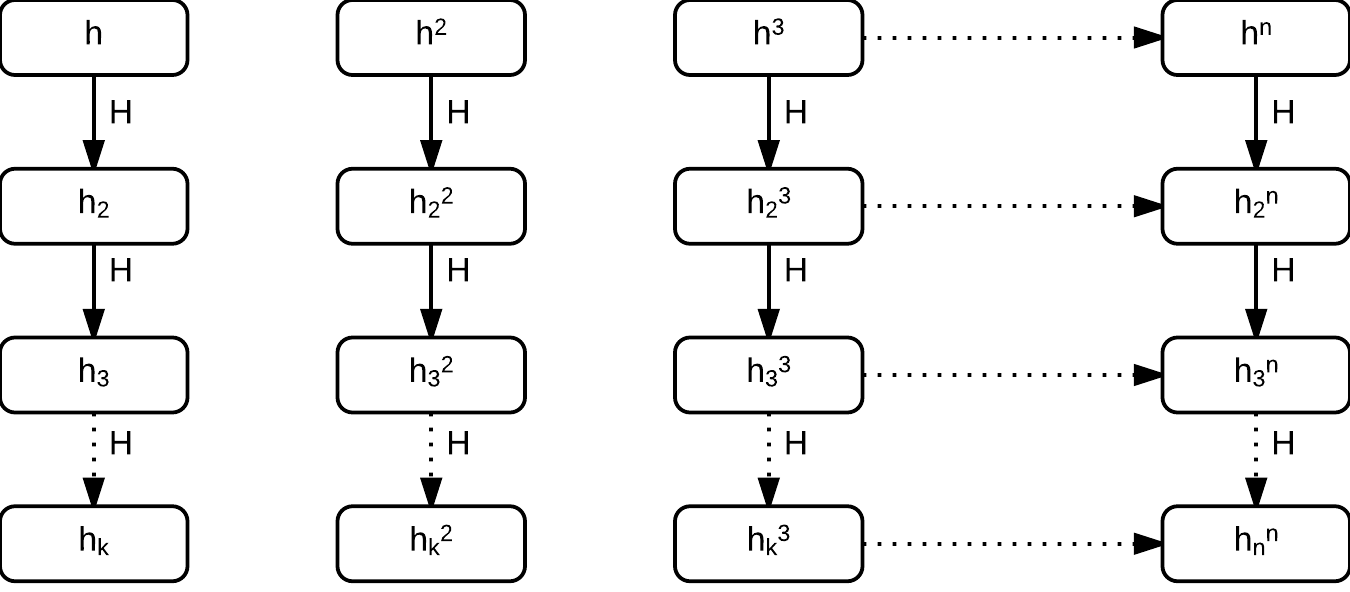
\includegraphics[width=\textwidth]{rainbow-table}
    \caption{Rainbow table.}
    \label{rainbow-table}
\end{figure}


\subsection{Offline-online Gap and Classifying of Accounts.}\label{classification} Florêncio et al.~\cite{guide-pws} shows that a password have to be able to withstand at least $10^6$ guesses to be safe against online attacks. To survive offline attacks at least $10^{14}$ would be necessary. The point highlighted is that a password able to withstand $10^{10}$ guesses, is no more likely to survive a offline attack than a password only protected against $10^6$ guesses. 
\par They suggest that users should classify all accounts into categories ranging from ``Don't-care'' to ``Ultra-sensitive''. The idea is that it is no point in using complex and long password on an account which doesn't contain any sensitive information. For critical accounts related to finance, primary employment or other highly confidential documents it is advised to use multiple factors of authentication~\cite{2-factor-auth}. Accounts used for e.g. social media or streaming would probably be categorized as ``medium-consequence'' as loss of such accounts would be more about time and effort, than financial loss. It is of course up to the users to categorize how critical it would be to lose each account (see ~\cite{guide-pws} for an example category division). 
\par The important point is that accounts should be treated differently, there is no point in using a 20 characters long password on an online chess game account, while it would be reasonable on a online banking account. This can be utilized to make password management more adaptable and easy to use. Especially when using a password management scheme, as the one evaluated in this project, it is very beneficial to lower the average length of passwords, while still having long passwords for the important accounts. This will be utilized to improve the usability of the scheme implemented later.

%\section{The User}\label{sec:the-user}
%"Good passwords" as discussed in \ref{password-strength} does not go well with the human memory. The first limitation which will be an important property later are the limitation to how much data we can store in immediate memory, this limit was showed to be 7 chunks of data at once~\cite{magic-seven_miller}. This data can not be from a random selection which is what a good password requires.   


\section{Password Management}
As seen in the previous sections passwords introduce a dilemma as passwords are supposed to be hard to ``guess'' and thus hard to remember. The naive solution to this problem is to either use one password for many accounts or to write down passwords. To make the process of managing passwords easier, several techniques and tools have been suggested~\cite{management-strategies}. Examples are reminder features including the ``I forgot my password''-function most websites implement, browser cookies allowing users to stay logged in across browser sessions or services storing the passwords. These are all ``computer aided'' tools, which will store or keep users logged in without actually having to remember the password. This usually limits the users to stay on the same machine while using the account, this way users will probably forget passwords and be forced into using the ``forgot my password''-function eventually. A different approach is to use a technique to actually remember the passwords without storing them.
\par Consider a password management scheme to be a method helping users remember password without actually storing them. The term password management software or password mangers are used about solutions which store the passwords in some way.

\subsection{Password management schemes}
 
Password creation and memorization techniques assists users in remembering passwords, trying to circumvent the limitations of the human memory~\cite{human-memory}. 
\par Blocki et al. \cite{naturally-rehearsing} consider 4 different examples of password managements schemes to illustrate how users might choose and remember their passwords.
\begin{itemize}
    \item{ Reuse Weak. } When users select a random phrase or word $w$ and reuse this as the password $p_i=w$ for all accounts. While maybe not very strong, this is the most simple example of a password management scheme.
    \item{ Reuse Strong. } Same as reuse weak but users chose four random words $w_1,w_2,w_3,w_4$ and reuse the concatenation of these as the password $p_i = w_1w_2w_3w_4$ for all his accounts.
    \item{Lifehacker.} Users chose three random words $w_1, w_2, w_3$ as a base password $b=w_1w_2w_3$ as well as a derivation rule $d$ used to derive unique data from the site names for each password \footnote{How to Update Your Insecure Passwords and Make Them Easy to Use - \url{http://lifehacker.com/5631203/how-to-update-your-insecure-passwords-and-make-them-easy-to-use}}. Example of a derivation rule could be the first and last three letters of the service name. The password for account $A_i$ would then be $p_i = b d(A_i)$ with $d(A_i)$ being the string derived from the site name. In practice a password generated using the method might look like "facthreerandomwordsook". 
    \item{Strong Random and Independent.} Users chose new words $w^i_1, w^i_2, w^i_3, w^i_4$ for each account to be used as passwords $p_i = w^i_1w^i_2w^i_3w^i_4$.
\end{itemize}
It is clear that the three former schemes are much easier to use than the last one. Most users would prefer the first ones because they do not require much, if any, rehearsal while the one strong scheme would require too much effort in terms of rehearsing and memorization. This trade-off between usability and security is the main problem when designing password management schemes. For a scheme to be popular it cannot require too much extra rehearsal, while a secure scheme most of the time will require some.



\subsection{Password manager software.} \label{subsec:pms}
Applications meant to keep passwords safe the for users. These applications can either be stand alone programs or, more common, browser extensions such as LastPass \footnote{LastPass - \url{https://lastpass.com/}}. LastPass provide an user interface to generate and store passwords for online services, as well as form fillers to enter them when logging in. The passwords are encrypted using a master password protecting the user credentials against both server leakage and insiders accessing the data. Such systems usually provides a lot of extra features such as automatically changing of passwords and syncing between devices. 

\paragraph{Built-in browser password managers.} Most modern browsers provide "remember password" functions. These functions act similar to software like LastPass, by storing the users' passwords in some fashion, then reproduce it when login in. 

These kinds of systems and applications require the users to trust that the implemented systems are secure enough to prevent adversaries, both insiders and outsiders, from stealing credentials. Software aiding the users by storing passwords often also provide autofill-functions, automatically filling in the username and password of the associated site. Silver et al. \cite{pw-managment-attacks} propose attacks exploiting these autofill functions to extract passwords from the password manager, the most basic example attack is shown in example \ref{rouge-wifi}. Despite the obvious weaknesses in many password managers, they still argue that password managers can strengthen credential security if implemented correctly.  
\begin{example}\label{rouge-wifi}
    Consider users connecting to a open wifi at a coffee bar or another public place. It is not unusual to present the users with a ``landing page'' asking for approval of some usage agreement. The rouge wifi provider could include multiple iframes\footnote{\url{Iframe - http://www.w3schools.com/tags/tag_iframe.asp}} pointing to the login pages of common sites the users probably have stored credentials for. See figure \ref{rouge-wifi-page}. By injecting Javascript in the iframes the attacker can extract all the usernames and passwords autofilled by the password manager. Note that the iframes displayed in the figure are not visible to the users, to them it looks like a standard landing/welcome page. Silver et al. \cite{pw-managment-attacks} claim that six out of ten password managers were vulnerable to this simple attack.


\begin{figure}
    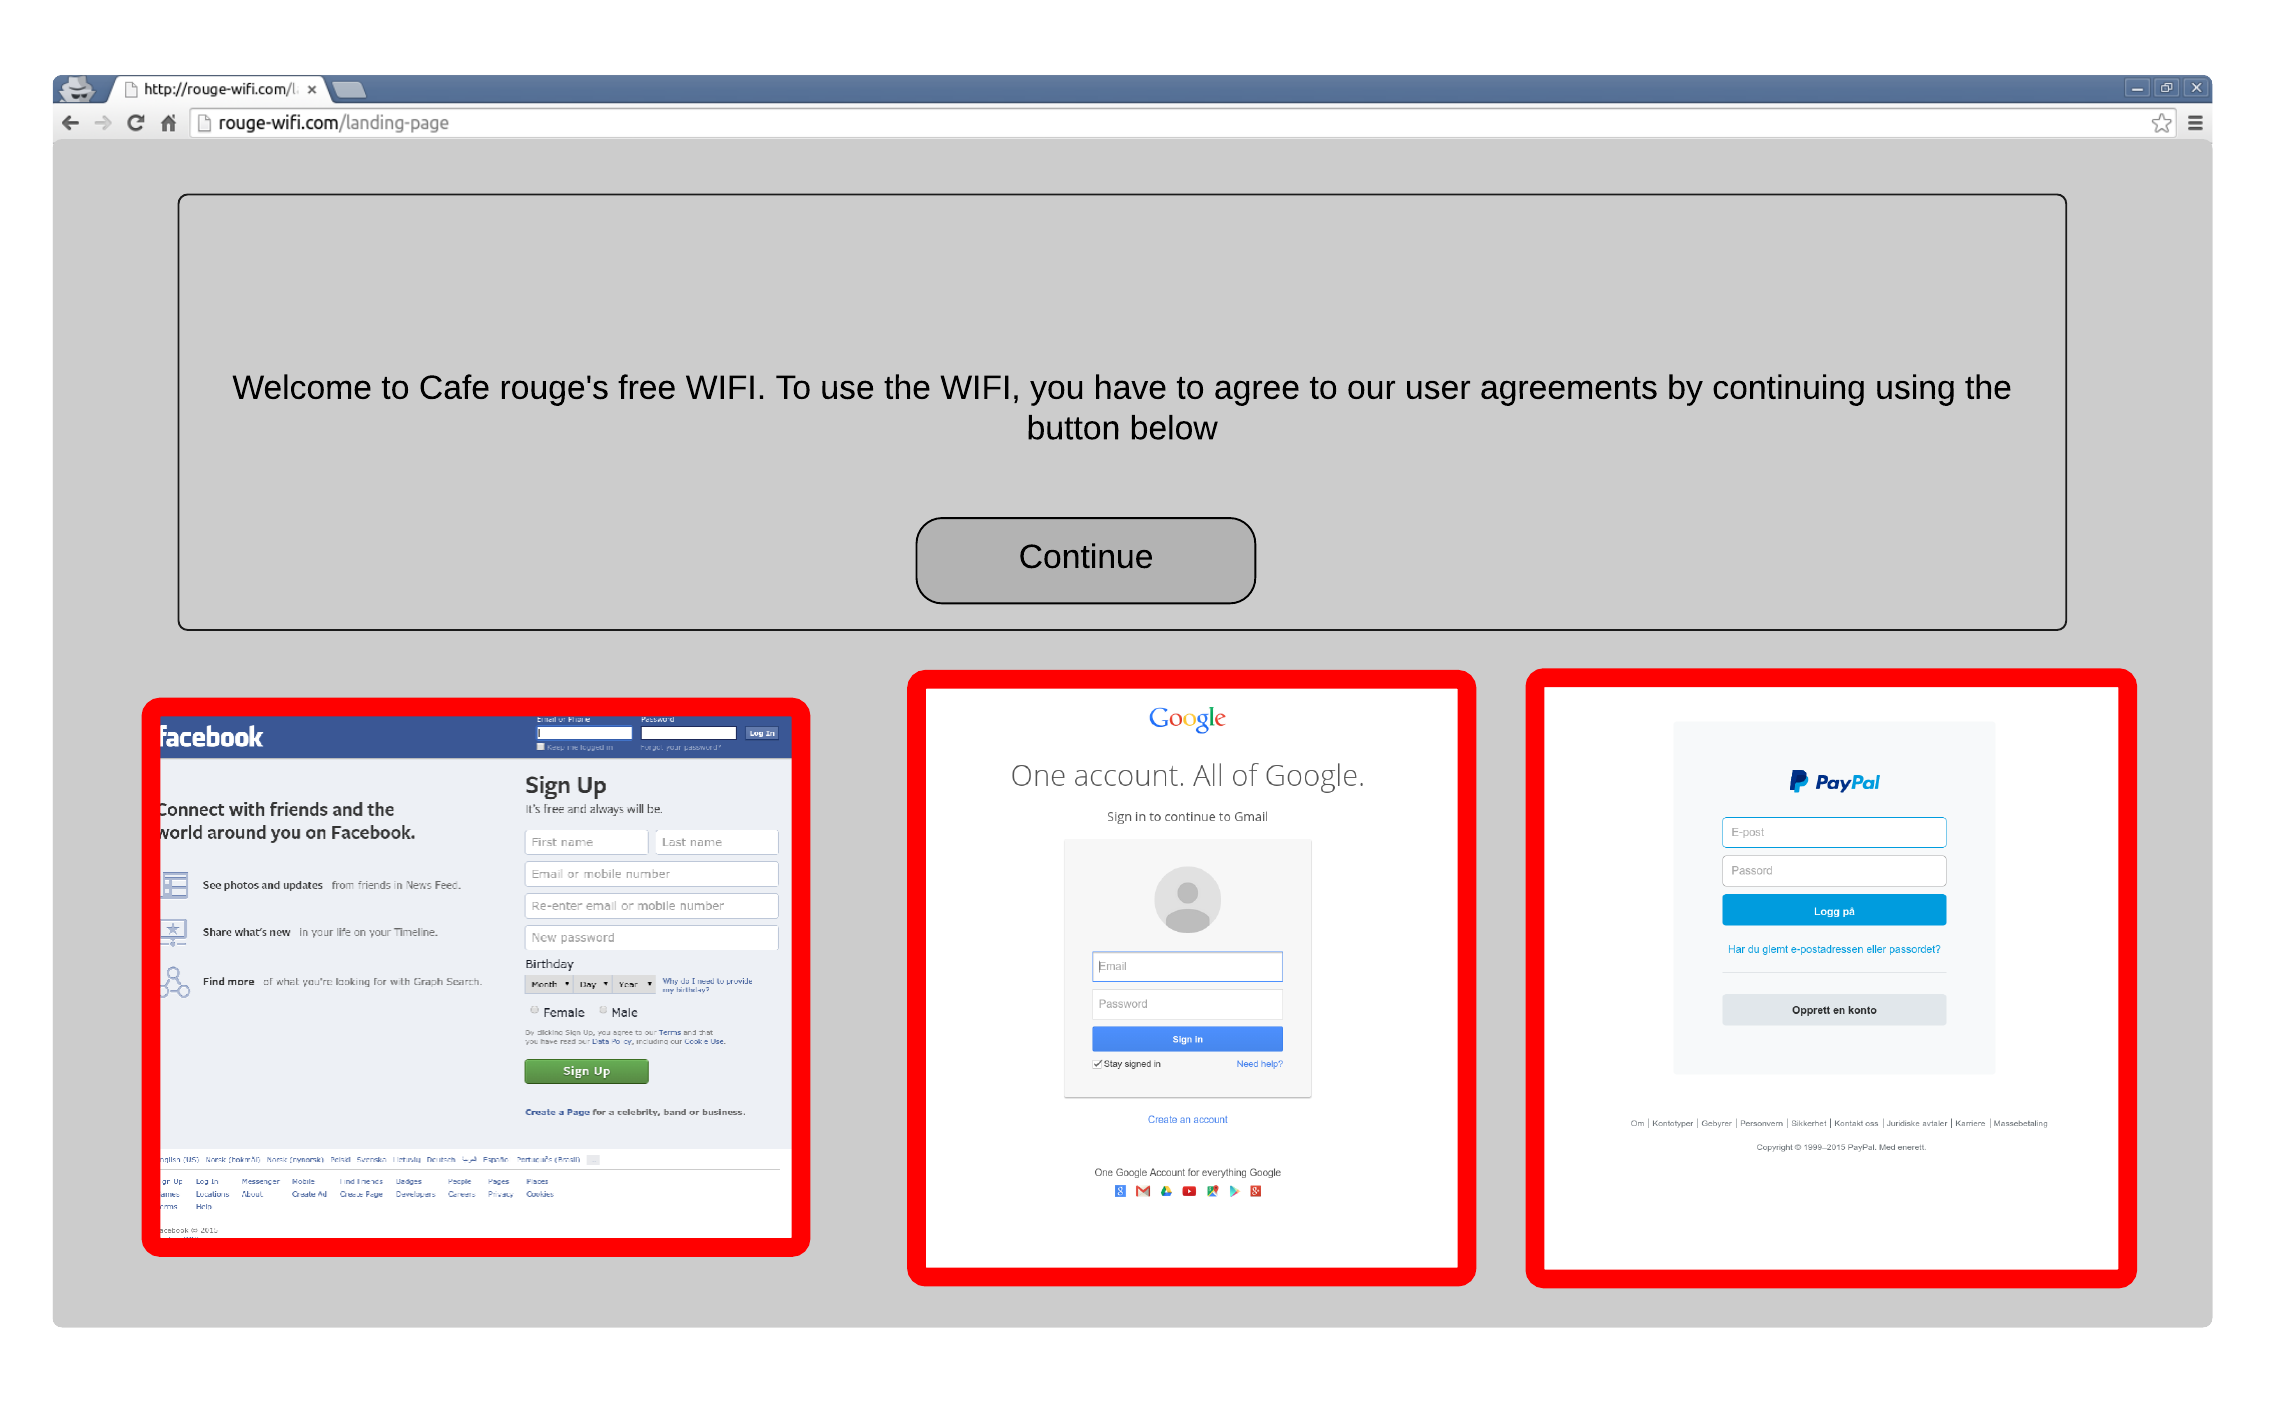
\includegraphics[width=\textwidth]{rouge-wifi-page}
    \caption{Rouge wifi landing page containing iframes with common sites, used to steal password from an autofilling password manager.} 
    \label{rouge-wifi-page}
\end{figure}

\end{example}

\par Even if the password manager is secure against autofill-attacks, or if it does not include the feature, the manager might still be at risk. If the account storing all the usernames and passwords where to be compromised, all the sites would be compromised, so it is important that the password manager is even more secure than the sites themselves. 
\par Zhao et al. \cite{lastpass-security} identified several vulnerabilities in the LastPass implementation, even though no known breaches has been reported. They investigate different types of attacks, including attacks on local decrypted credentials; request monitoring attacks which tries to intercept request between the password manager and related cloud-storage; as well as brute-force attacks trying to crack the master password. The conclusion is that password managers are double-edged swords, in theory they help make password authentication stronger, but if implemented slightly wrong may be a major vulnerability. Storing all the passwords at one place makes a obvious point of attack for adversaries since breaking the manager most of the time would break all accounts stored within.





%\section{Usability Model}\label{sec:usability-model}
%This section presents the usability model defined by Blocki et al. \cite{naturally-rehearsing}, which predicts the efforts required of users to keep a set of secrets memorized without forgetting it. It will be presented in the context of password management schemes, in particular the HCP scheme relied on in this project. The model will later be used to analyze the usability of the scheme and related applications.
%
%\subsection{Definitions}
%A password management scheme generates and keeps track of passwords $p_1, \dots, p_m \in P$ for all $m \in A$ accounts of users. $P$ is all possible passwords. Let $(\hat c, \hat a)$ represent an association between an object (e.g. letter or picture) and a related  mapping (typically a digit between 1 and 10). Users have to rehearse the association $(\hat c, \hat a)$ to avoid forgetting it. Next two schedules are defined defining how often users have to rehearse to not forget a association, and how often they visit an account.
%
%\begin{definition}\label{rehearsal-schedule}
%    \cite{hcp-blocki} A rehearsal schedule for an object-mapping association $(\hat c, \hat a)$ is a series of points in time $t^{\hat c}_0 < t^{\hat c}_1 < \dots$. A rehearsal requirement for each $i \ge 0$ says that the object-mapping association pair must be rehearsed at least once in the time interval $[ t^{\hat c}_i, t^{\hat c}_i+1) = \{x \in \mathbb{R} \vert t^{\hat c}_i \le x < t^{\hat c}_{i+1} \} $.
%\end{definition}
%A rehearsal schedule as defined in definition \ref{rehearsal-schedule} is said to be sufficient if a user can keep an association in his memory without forgetting by following the schedule.
%
%\paragraph{Visitation schedule \cite{hcp-blocki}} is a series of numbers $\tau^i_0 < \tau^i_1 < ...$ representing the points in time when a user visits account $A_i$. This schedule cannot be known exactly so it is modeled using a random process with a parameter $\lambda_i$ based on the average time between visits to account $A_i$ - $E[\tau^i_{j+1} - \tau^i_j]$.
%\par A rehearsal requirement can also be satisfied naturally if a user visits an account using the object $\hat c$ during the interval $[ t^{\hat c}_i, t^{\hat c}_i+1)$, as defined in definition \ref{natural-rehearsal},
%
%\begin{definition}\label{natural-rehearsal}\cite{hcp-blocki}
%     A rehearsal requirement $[ t^{\hat c}_i, t^{\hat c}_i+1)$ is naturally satisfied by a visitation schedule $\tau^i_0 < \tau^i_1 <\dots$ if for any $j \in [m]$ and $k \in \mathbb{N}$ so that $\hat c \in c_j$ and $\tau^j_ki \in [ t^{\hat c}_i, t^{\hat c}_i+1)$. Let \\
%    \begin{large}
%    \centerline{ $ER_{t,\hat c} = \vert\{ i \vert t^{\hat c}_{i+1} \le t \wedge \forall j ,k.(\hat c \notin c_j \wedge \tau^j_k \notin [t^{\hat c}_i, t^{\hat c}_i))\} \vert$ }
%    \end{large}
%    denote how many extra rehearsals required, that are \emph{not} satisfied by the visitation schedule, during time time interval $[0,t]$
%\end{definition}
%
%
%
%
%\subsection{Model}
%The core of the model is that usability depends on rehearsal required to remember all passwords, relative to the visitation schedule of the specific user. How hard it is for any given user to remember a relation between object may vary from person to person depending on mnemonic technique and genetic conditions. This is adjusted for in the model by the constant $s$ representing the combined strength of mnemonic technique and the memory of a user. Next, consider two different rehearsal requirements specifying what is needed to maintain a memory.
%
%\begin{requirement}\label{CR}
%    \textbf{ Constant Rehearsal Assumption (CR)\cite{naturally-rehearsing}.} The rehearsal schedule given by $R(\hat c, i) = i s$ is sufficient to maintain the association $(\hat c, \hat a)$ in memory.
%\end{requirement}
%
%\begin{requirement}\label{ER}
%    \textbf{Expanding Rehearsal Assumption (ER)\cite{naturally-rehearsing}.} The rehearsal schedule given by $R(\hat c, i)=2^{i s}$ is sufficient to maintain the association $(\hat c, \hat a)$ in memory.
%\end{requirement}
%
%The difference between these two assumptions about human memory is that CR assumes that users have to keep rehearsing every $s$ days for as long as they want to make sure to not forget anything. This might be too pessimistic since it is reasonable to assume that it gets easier to rehearse for each rehearsal. This is what ER assumes, if a relation has been rehearsed $i$ times it does not have to be rehearsed again in $2^{i s}$ days. ER is the most intuitive assumption to make and is backed up by experiments on how the human brain forgets over time \cite{forgetting, human-memory}.
%
%\par 
%\subsubsection{Visitation Schedule}
%Every user will eventually have a unique visitation schedule which will vary greatly from user to user. The model uses a Poisson process to model the visitations schedule for a given site $A_i$, with parameter $\lambda_i$. The average time between visits,$\frac{1}{\lambda_i}$, is assumed to be known for each visitation schedule. A site visited every day would yield $\lambda_i = 1$ day, and $\lambda_i=\frac{1}{365}$ days for a site visited annually. 
%\par Next, the model uses four different types of users which may have accounts of 5 different account types based on visitation frequency. The users can be: very active, typical, occasional or infrequent, while an account can be visited daily, every three days, every week, every month or annually. Table \ref{users} defines how many of each type the users have respectively. For example, active users are said to have $10$ accounts they visit daily and $35$ visited annually.
%
%\begin{table}
%    \centering
%\begin{tabular}{|c||c|c|c|c|c|}
%    \hline
%    Visitation schedule & 1 & $\frac{1}{3}$ & $\frac{1}{7}$ & $\frac{1}{31}$ & $\frac{1}{365}$ \\
%    \hline \hline
%    Very Active & 10 &10 &10 &10 & 35 \\
%    \hline
%    Typical & 5 & 10 & 10 & 10 & 40 \\
%    \hline
%    Occasional & 2 & 10 & 20 & 20 & 23 \\
%    \hline
%    Infrequent & 0 & 2 & 5 & 10 &  58 \\
%    \hline
%\end{tabular}
%\caption{Visitation schedules.}
%\label{users}
%\end{table}
%
%\subsubsection{Extra rehearsals}
%If an object-mapping association $(\hat c, \hat a)$ is not rehearsed through normal usage within the interval $[t^{\hat c}_i, t^{\hat c}_{i+1})$ users would have to rehearse the association to prevent forgetting it. $ER_{t,\hat c}$ in definition \ref{natural-rehearsal} gives the number of extra rehearsals of $(\hat c, \hat a)$ in a given time interval. From this it can be seen that $ER_t = \sum_{\hat c} ER_{t, \hat c}$ gives the number of rehearsals, in addition to natural rehearsal, needed to maintain all objects in a set of associations. In the context of a password management scheme it is clear smaller values for $E[ER_t]$ yield less effort required by the users.
%\par Blocki et al.\cite{naturally-rehearsing} proves that, given a sufficient rehearsal schedule  and a specific visitation schedule, $ER_t$, total number of extra rehearsals needed to keep all object-mappings in memory, can be predicted through theorem \ref{ERt}. 
%
%
%\begin{theorem}\label{ERt}
%    \cite{naturally-rehearsing} Let $i_{\hat c}* = (arg max_x t^{\hat c}_x < t)- 1 $, then 
%
%    $ E[ER_t] = \sum_{\hat c \in C} \sum^{i_{\hat c *}}_{i=0} exp\bigg(-\bigg(\sum\limits_{j:\hat c \in C_j} \lambda_j \bigg)(t^{\hat c}_{t+1} - t^{\hat c}_i)\bigg)$
%\end{theorem}
%
%\begin{lemma}
%    \cite{naturally-rehearsing} The probability that $\hat c$ is not rehearsed naturally during the interval $[a,b]$ is $exp(-\lambda_{\hat c} (b-a))$, given $S_{\hat c} = \{i \vert \hat c \in c_i \}$ and $\lambda_{\hat c}= \sum_{i \in S_{\hat c}}$
%\end{lemma}
%
%
%













\chapter{Human Computable Passwords}


\section{Password Managment Scheme}

\subsection{Human Computable Functions}


\section{Usability and Security Challenges}




\chapter{Application}\label{app}
This chapter will describe how browser extensions are built in google chrome, focusing on architecture and security features. Browser extensions can be utilized to build an application implementing "human computable passwords" as described in \autoref{ch:hcp}. The scheme is different from other traditional password managers since it does not \emph{store} the password, but challenges \emph{helping} the user to remember strong passwords. The idea by using browser extensions to implement this is to have an extension monitor the password fields of the sites a user visits and update the challenges depending on the current state of the active site. This technique will be described and a prototype extension demonstrated. 
\section{Browser Extensions}\label{browser-extensions}
Modern computer users shift towards doing more and more work through their web browsers. Web applications have become popular due to the ubiquity of browsers, thus allowing web apps to run anywhere. A web app can run at any platform running a web browser, allowing the application to run on multiple platforms as well as different devices. Updates can be applied quickly without having to distribute patches to a possibly huge amount of devices.
\par Browser extensions add additional features to the web browser allowing the user to tweak the experience of the web pages visited. Typical examples are extensions adding to, or tweaking already present features of the browser such as changing how bookmarks are managed, or adding additional features such as blocking advertisements. Lately browser extensions have been extended even further allowing standalone applications to be developed running as native applications \footnote{A new breed of Chrome apps, \url{http://chrome.blogspot.no/2013/09/a-new-breed-of-chrome-apps.html} - accessed: 2015-03-02}. This allows developers to create desktop apps using the same technology as in web apps, mainly HMTL5, Javascript and CCS.
\par This chapter will present Google chrome browser extensions, including architecture and security mechanisms.

%This project will utilize chrome extensions to create a password manager running in the browser. 
%The user interface will be in a panel spawned by a browser action activated when the user click the icon in the navbar. 
%The user interface is built using the open-source web application framework AngularJS \cite{angularjs}, storage is done using the chrome local storage API.

\subsection{Extension Security}\label{extension-sec}
\par Browser extensions introduce some security concerns which must not be forgotten while developing applications using this environment. Chrome extensions run in the browser with access to both the \gls{dom} of the active page as well as the native file system and connected devices. The overall architecture of a chrome extension is summarized in \autoref{extension-architecture} and described in the chrome extensions documentation \footnote{What are extensions?, \url{https://developer.chrome.com/extensions/overview} - accessed 2015-03-02}. This section will describe the architecture considering security concerns relevant when developing chrome extensions which handle sensitive data such as passwords.

%The extension core consist of the actual application interface visible to the user as well as long running background jobs and business logic. The background page can be used to spawn panels or popups, and has access to browser APIs.  The extensions is activated through a icon in the browser navbar as seen in \autoref{extension-ux}. Clicking the icon typically spawns a popup or a panel to interact with the user. In addition to the core, each extensions can have content scripts which has access to the content of the current active web page, and can monitor and alter \gls{dom} of this. 


\begin{figure}[h]
   \fbox{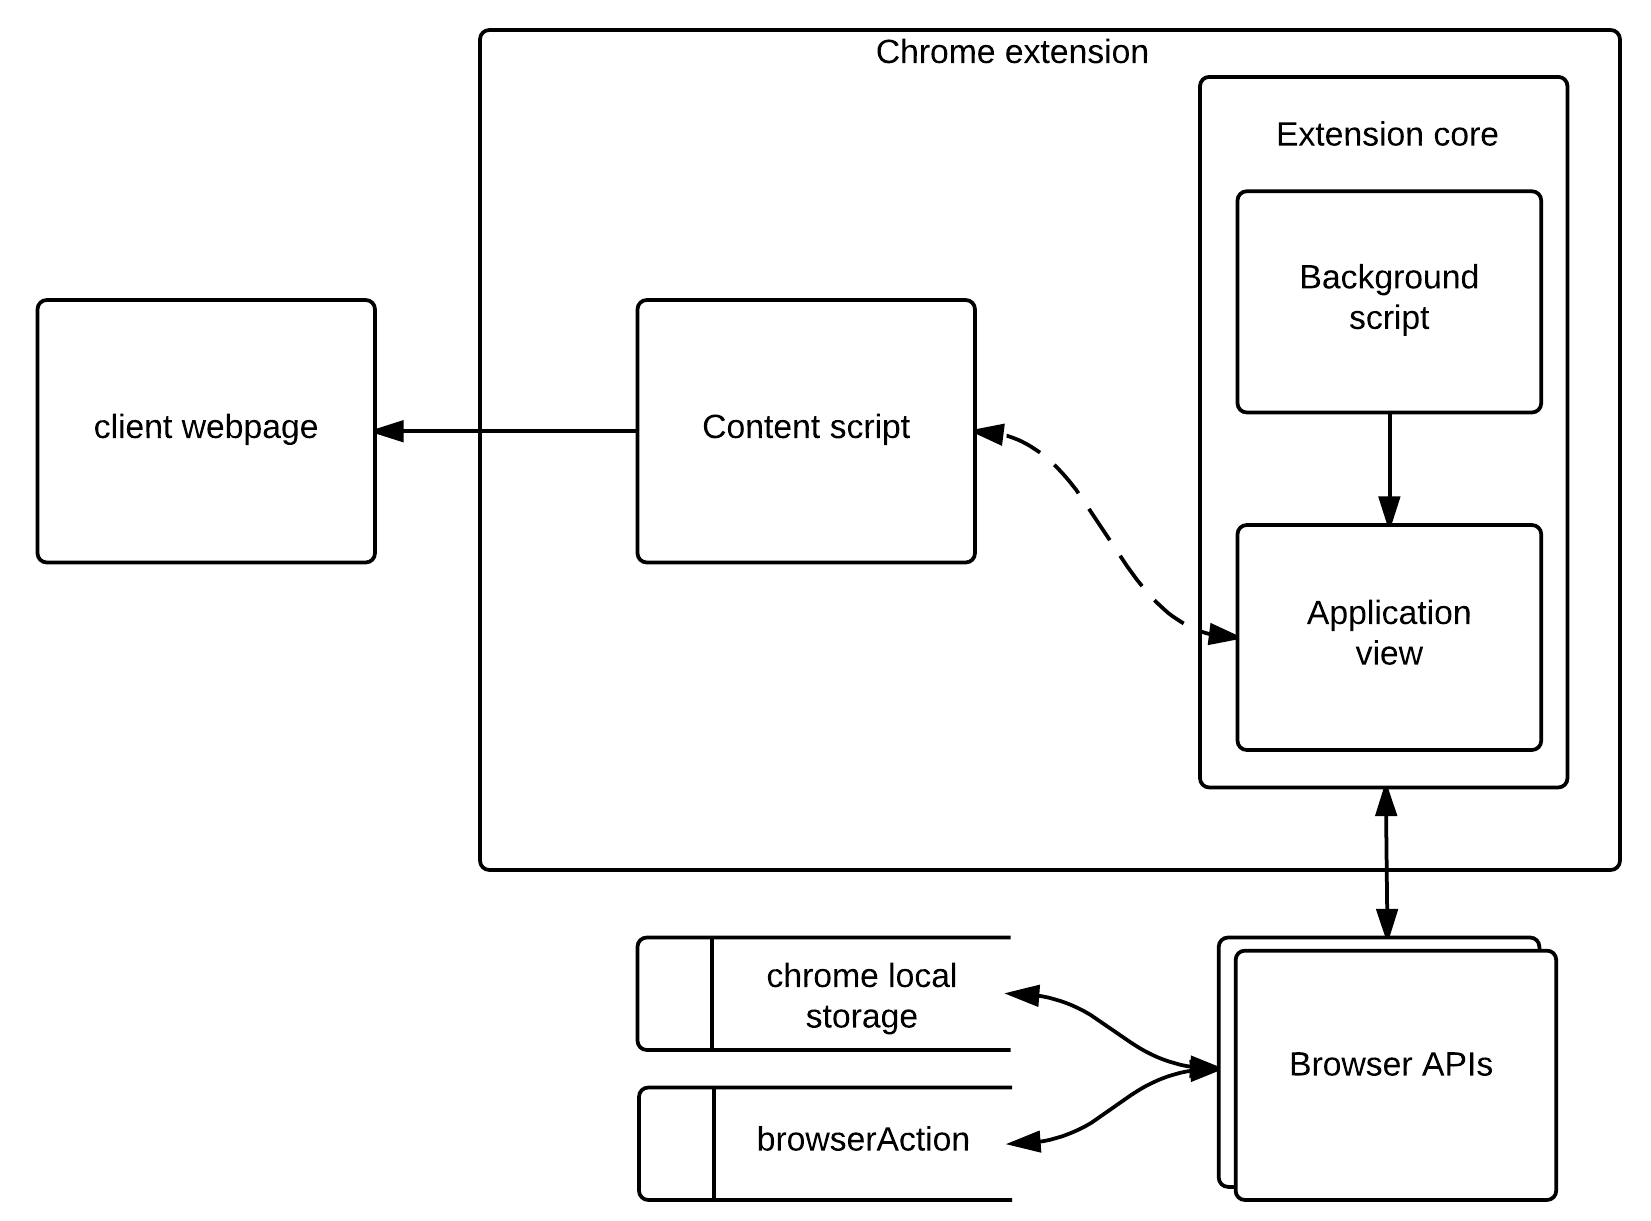
\includegraphics[width=\textwidth]{chrome-extension-architecture} }
    \caption{Chrome extension architecture.}
    \label{extension-architecture}
\end{figure}

\par Earlier extensions written for IE and Firefox ran in the same process as the browser and shared the same privileges. This made extensions an attractive entry point for attackers, since a buggy extension could leave security holes leaking sensitive information or even provide an entry point to the underlying operating system. For these browsers several frameworks for security have been proposed \cite{firefox-ie, js-info-flow}, trying to mitigate vulnerabilities is browser extensions. The chrome extensions architecture is built from scratch with security in mind. Chrome uses a permission system following three principles \cite{liu-chrome}; \emph{least privileges}, \emph{privilege separation} and \emph{process isolation}. 

\paragraph{Least privilege} specifies that extensions should only have to privileges they need functions, not share those of the browser. The privileges of each extension are requested in the \emph{manifest} file \footnote{Manifest file format, \url{https://developer.chrome.com/apps/manifest} - accessed 2015-03-04}. This json file needs to be included in all chrome extensions, and consist of all the permissions needed by the extension as well as some meta data and version information. This is done to prevent compromised extensions from exploiting other permissions than those available at runtime. An example of a manifest file can look like this: 

\begin{verbatim}
{
    "name": "Example extensions",
    "description": "An example extensions to demonstrate how the
                    manifest file works.",
    "version": "1.2",
    "manifest_version": "2"
    "background_page": "main.hmtl",
    "permissions": [
        "bookmarks",
        "storage",
        "https://*.ntnu.no"
    ]
}
\end{verbatim}
This extension has specified access to the bookmarks API, chrome local storage and all sub domains of ntnu.no. Extensions can request different permissions in the manifest file including web site access, API access and native messaging. If an extension contains weaknesses it will not compromise any other parts of the system not covered by the specified privileges. For the least privileges approach to work properly each developer should only request the permissions needed, Barth et al. \cite{protecting-browsers} examined this behavior and concluded that developers of chrome extensions usually limit the origins requested to the ones needed. 

\paragraph{Privilege separation.} Chrome extensions are, as mentioned, divided into components; content scripts, extension core and native binaries. The addition of native binaries allows extensions to run arbitrary code on the host computer, thus posing a serious security threat. This project does not use this permission, this component will thus not be mentioned from now on. 
\par \emph{Content scripts} are javascript files allowing extensions to communicate with untrusted web content of the active web page. These scripts are instantiated for each visited web page and has direct access to the \gls{dom} of these, allowing both monitoring and editing of DOM elements. To be able to inject content scripts to a visited page, the origin of the site has to be added to the manifest file. Other than this permission, content script are only allowed to communicate with the extension core. It is important that the privileges of these scripts are at the minimum level since they are at high risk of being attacked by malicious web sites \cite{chrome-extension-dangers}, due to the direct interaction with the \gls{dom}. 
\par The \emph{extension core} is the application interface responsible for interaction with the user as well as long running background jobs and business logic. The core is written in HTML and javascript and is responsible for spawning popups and panels, as well as listening for browser action. The typical way to activate a extensions is by clicking an icon in the navigation bar, which then activates either a popup or a detached panel. The core is the components with the most privileges as it does not interact with any insecure content directly, only through direct messaging to a content script or using http requests if the target origin is defined in the manifest. 
\par In addition to this the core has access to the extension APIs, these are special-purpose interfaces providing additional features such as alarms, bookmarks, cookie and file storage. The APIs are made available through the manifest file and only those specified there can be used. \autoref{extension-ux} illustrates the interaction between the background page, content scripts, panels and active web page. The information flow starts by clicking the extension's icon in the navigation bar which launches the background page spawning a panel in the browser. A content script is injected in the current web site (google.no in the example), the script now have access to the DOM of this site and can communicate with the background which in turn can update the panel. 


\begin{figure}[h]
    \fbox{ 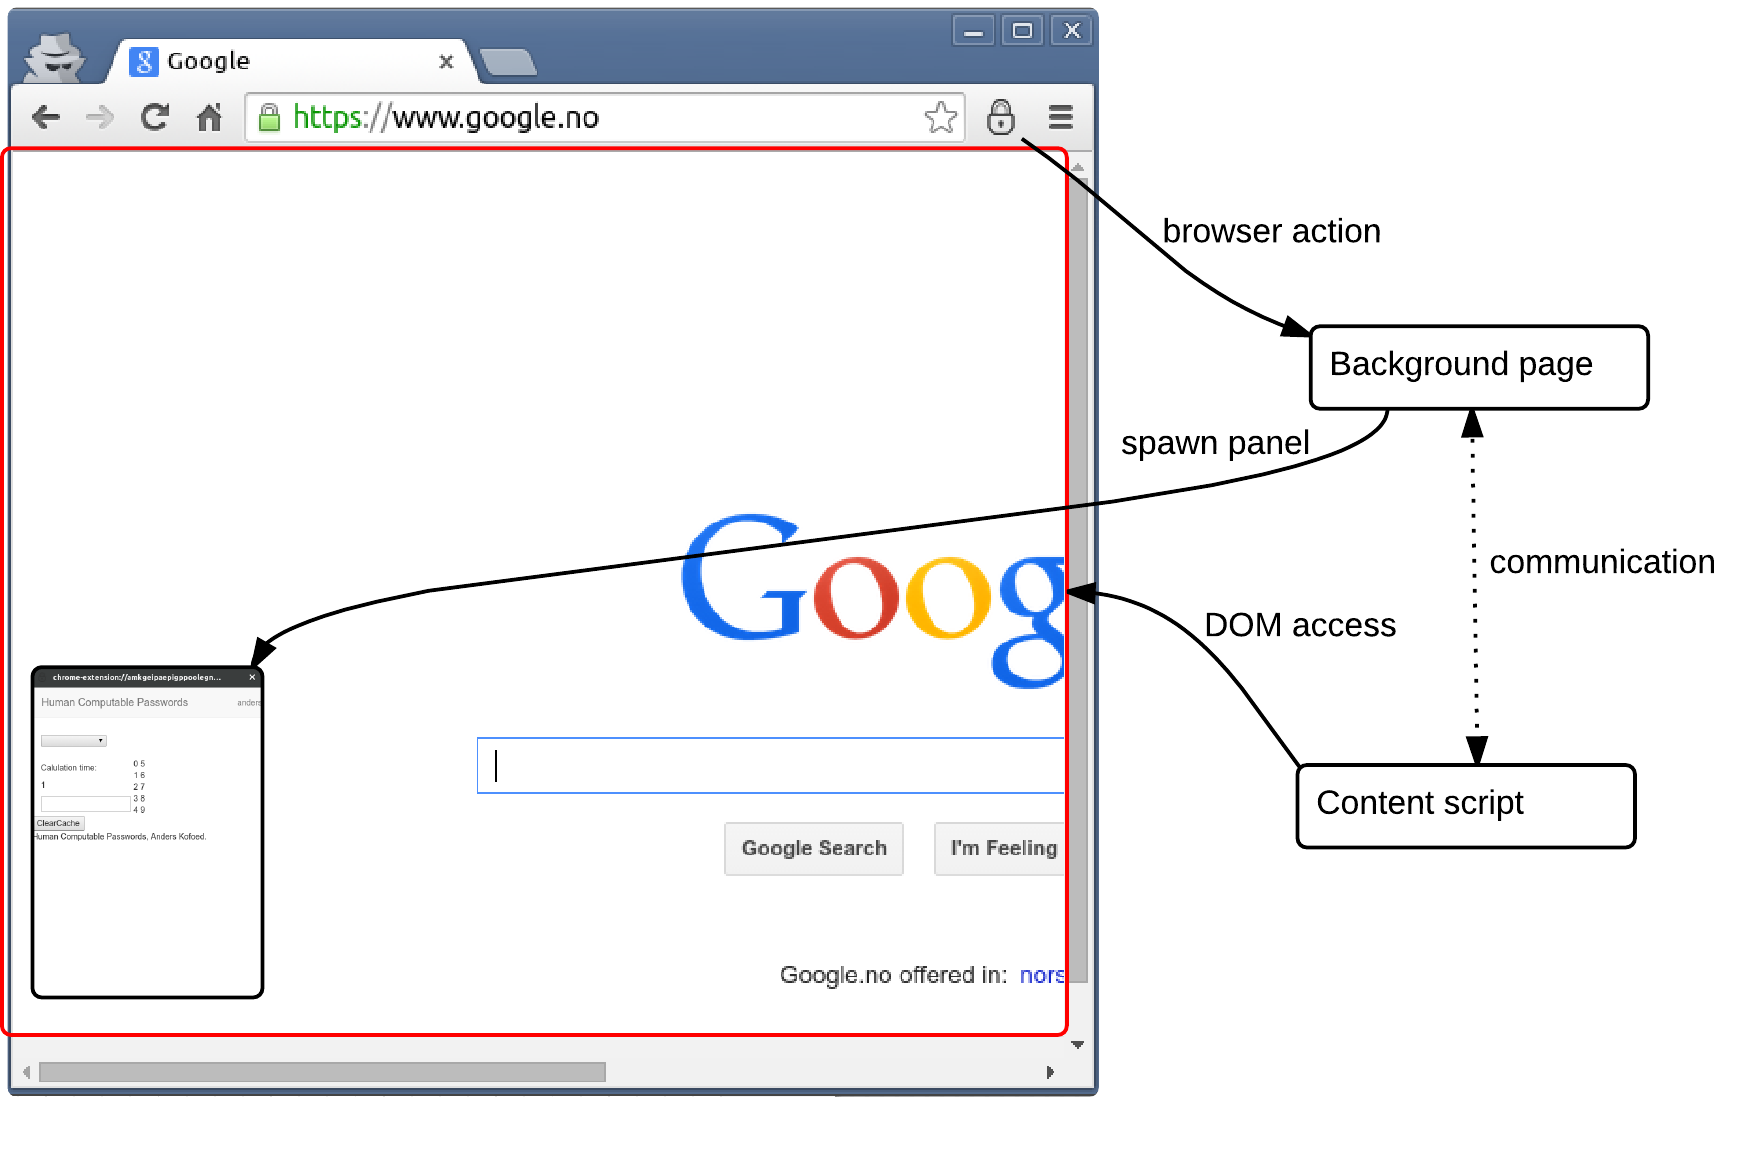
\includegraphics[width=\textwidth]{chrome-extension-ux} }
    \caption{Chrome extensions browser action and content scripts.}
    \label{extension-ux}
\end{figure}

\paragraph{Process isolation} is a set of mechanisms shielding the component from each other and from the web. Usually when javascript is loaded from the web the authority of the script is limited to the origin from where the script is loaded \cite{protecting-browsers}. Since the scripts used by the extensions are loaded from the file system, they do not have a origin in the same sense, and thus need to be assigned one. This is done by including a public key in the url of the extension, allowing a packaged extension to sign itself, freeing it from any naming authority or similar. The public key also enables usage of persistent data storage, since the origin of the extension can stay the same throughout updates and patches. This wouldn't be possible otherwise since the chrome local storage API relies on origin. Each extension will have a private/public key pair, a hash of the public key is used as id and each updated version uploaded will be sign with the private key. By doing this the id stays the same throughout versions and can be verified by when uploading and by chrome storage after releasing a new version. 


\par The different components also run in different processes. The content scripts are injected and ran in the same process as the active web page, while the core run in its own process started when the extension is initiated. This protects against javascript injections from malicious web sites\cite{javascript-injection}. Since the content script executes in the same environment as the active web page, users may visit websites hosting content meant to exploit extensions\cite{carlini-chrome}, possibly stealing sensitive information or issue fake requests.
\par Finally content scripts are ran in a separate javascript environment isolating it from the possibly insecure environment of the web site. The environment of the content scripts are called isolated world, which in practice is a separate set of javascript objects reflecting the ones of the underlying DOM of the web page. This means that the content script can read and edit the DOM of the page it is injected into, but not access variables or javascript functions present in the web page. Both the page and the content scripts sees no other javascript executing in their own isolated world, but they share the same DOM \footnote{Content Scripts, \url{https://developer.chrome.com/extensions/content_scripts} - accessed: 2015-03-05}.


\section{Human Computable Passwords Chrome Extension}
Chrome extensions are very useful in that they can be ran from any computer with Google chrome installed, thus on any operating system and on any computer. An extension makes it possible to run applications while browsing the web, which in the case of an password management scheme is very useful. An application meant to help the user recall complex passwords should preferably be visible simultaneously with the password field. Popular password management software today are usually either web applications, mobile applications or native desktop applications\footnote{Five Best Password Managers. \url{ http://lifehacker.com/5529133/five-best-password-managers }}, some of these might include plug-ins such as browser extensions. All of these password managers are reliably storing all the passwords as described in \autoref{subsec:pms}, then they are either auto-filled into the login fields or through copy pasting manually, which introduce several security issues\cite{protecting-browsers, javascript-injection, chrome-extension-dangers, carlini-chrome, liu-chrome, pw-managment-attacks}
\par This section will present the design and prototype implementation of the human computable password scheme (\autoref{ch:hcp}, \cite{hcp-blocki}. The design evolves around the fact that the scheme does not have to store anything securely, it is though important to make it as easy as possible for the user. The architecture will be similar to the one explained in \autoref{browser-extensions} using content scripts to monitor the password fields of the active browser session. The user interface will be presented through a "panel" in the browser. Panels are windows that stays in focus will interacting with other windows or applications \footnote{"Panels"- The Chromium Project. \url{https://www.chromium.org/developers/design-documents/extensions/proposed-changes/apis-under-development/panels}}.




\subsection{Applications Design}
The extension implementing human computable passwords \autoref{ch:hcp} will be an extension helping the user with storing and managing of challenges for different accounts. The generation of secret mappings will not be part of the application, this should be done through a separate program on the user's local computer. Such a program would follow algorithm \ref{gen-mapping}. The requirements for the extension are the following:

\begin{itemize}
    \item Provide an user interface making it easy for the user to calculate his password.
    \item The application should keep track of the active site, displaying challenges for the correct site without user interaction.
    \item Add new sites to the system easily. 
    \item The displayed challenge should update seamlessly while typing the password.
    \item The user should be able to type his password directly in the password field of the active site.
    \item If the user is about to forget a secret mapping, according to the usability model \ref{sec:usability-model}, the application should notify about it and advice the user to rehearse.
\end{itemize}


\subsubsection{AngularJs}
The front-end is built and updated using AngularJS\footnote{AngularJS, \url{https://angularjs.org/}}, which is an open source, client-side javascript framework. Angular is built using a variation of the model-view-controller architecture \cite{mvc}, though the creators of angular states that angular is a model-view-whatever framework\footnote{Model-View-Whatever - \url{ https://plus.google.com/+AngularJS/posts/aZNVhj355G2 }}, point being that what the architecture is called isn't important. 
\par The \emph{view}s in angular is templates written entirely in HTML, making it easy to read and update. The \emph{controller} contains all the business logic used by the view. The views and controllers are connected using a shared object called \emph{\$scope}, variables or functions on this object is usually defined in the controller and accessed by the view by using double curly brackets in the view (e.g. \{\{name\}\} to access the name variable on \$scope). Figure \ref{angular-data-binding} shows how scope is used to share variables between the controller and the view. 
See "Angular Essentials - Rodrigo Branas"\cite{angularjs-book} for a step-by-step introduction to AngularJS.

\begin{figure}[h]
    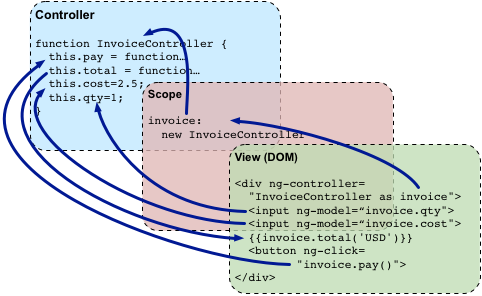
\includegraphics[width=\textwidth]{angular-data-binding} 
    \caption{Angular data binding with controller, view and scope. Figure from AngularJs developer guide.}
    \label{angular-data-binding}
\end{figure}


\par The main benefits of using angular in this project is the data-binding which makes it easy to update the HTML shown to the user. The extension will take advantage of this when updating the challenges seamlessly while the user calculates his password. The content of the extension will change according to the data filled in a password field without reloading the extension. 

\subsubsection{Chrome Storage.}\label{chrome-storage}
\emph{Local storage\footnote{Local storage - \url{ http://diveintohtml5.info/storage.html }}} is a way for applications to store data persistently and securely in the browser of clients. It is meant as an improvement of cookies which is the usual way of storing user data across sessions. The biggest problem with cookies is that they are sent with every HTTP request and thus slow down the applications using them. Local storage allows applications to store (key, value)-pairs in the browser. 
\par \emph{Chrome storage}\footnote{chrome.storage - \url{https://developer.chrome.com/extensions/storage}} is close to the same as local storage, differences being that chrome local storage allows applications to store data in what is called "chrome.storage.sync". This specific storage saves data locally, but also syncs it with the currently active chrome account, thus allowing a user to log into his account in any chrome browser and access the same application data. Chrome storage also allows storage of objects compared to local storage which only allows storing strings. This project will use chrome storage to persistently store challenges across sessions, and also provide backup. This way each user will be able to keep challenges for all their account within the storage of their google account. This is a important feature since it allows access to the challenges from remote locations as well.

\subsubsection{Content Scripts.}\label{cs}
Content scripts are javascript files running in the context of the active web page, as browsed by the user. These scripts has direct access to the content of the active site and can thus monitor and attach event listeners to the content of the page. The content scripts are isolated from the extension itself as describe in \autoref{extension-sec}, thus protecting the extension from possibly harmful sites trying to exploit weaknesses in the content script. Because of this the content scripts has to communicate with the extension through google chrome's built-in message passing system. Chrome message passing\footnote{Chrome message passing - \url{https://developer.chrome.com/extensions/messaging}} allows scripts to listen for and respond to messages. One side set up an event listener listening for messages, when a message is sent from the other side this event triggers and the message can be received and parsed. 
\par The content scripts and the message passing system are likely points of attack for adversaries. The content script can monitor the value of the password field and thus, in theory, steal these if a malicious script was able to trick it into leaking theme. The communication channel is not particularly prone to attacks since even if an adversary eavesdropped all data sent on it, the only information leaked would be the current length of the password. It is though important that the design is like this since the mistake of sending the whole password string, which might seem like a solution, would be potentially dangerous. 
\par Typical usage of content scripts in this application will be to attach event listeners to the password fields of the pages visited by the user, and message the extension when the value of the password field changes. When a change happens, the content script send a message containing the current length of the typed password, so that the extension can display the correct challenge. In example if the user has entered 4 characters of his password the extension should display the 5th challenge etc. The content script also keep the extension updated on the URL of the current page, by sending a message every time a page is loaded. The extension then displays the challenges corresponding to the password of that site. If the site does not have challenges stored by the application, the user can generate new ones and store these in the system through clicking a button.  

\subsection{User interface}
The user interface will be very simple, there will be two possible screens displayed to the user. Either, challenges associated to the current page will be shown, or a dialog asking the user to generate new challenges. The most important feature of the user interface is that it will automatically update depending on what site the user is currently browsing, and display the correct challenge when typing passwords. Wireframes illustrating the page schematics of the extension are shown in figures \ref{add-new-screen} and \ref{challenge-screen}.

\begin{figure}[h]
    \centering
    \begin{subfigure}[t]{0.49\textwidth}
        \centering
        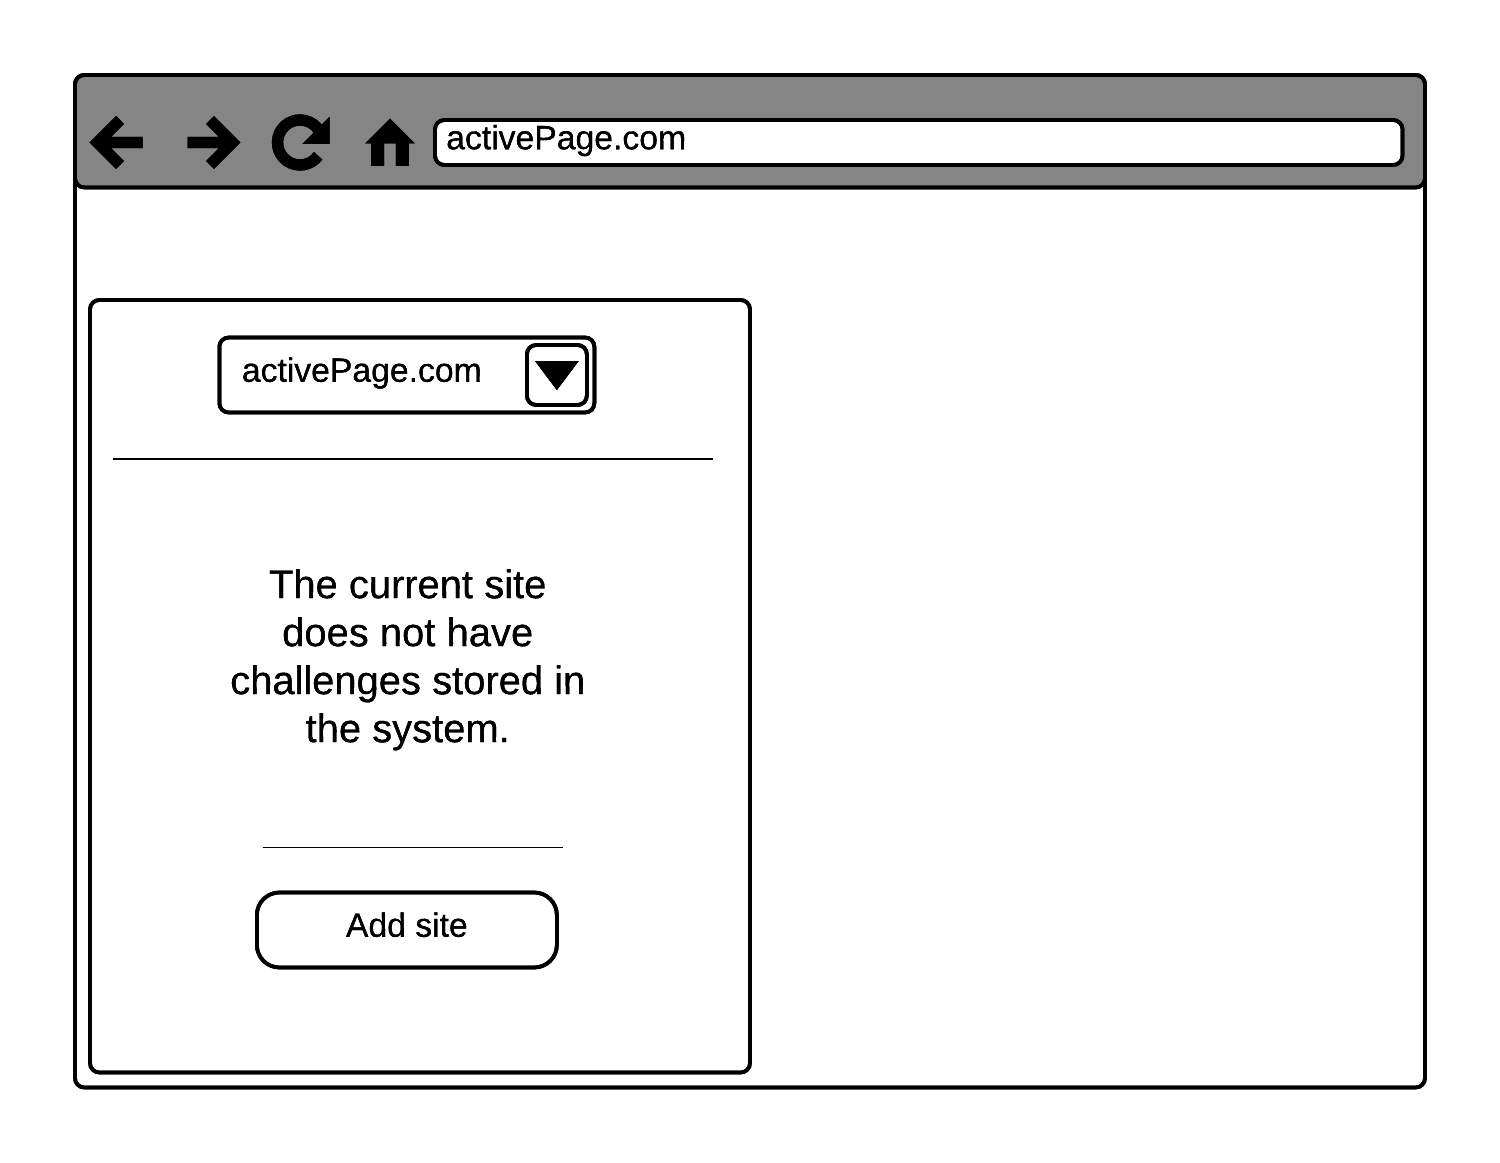
\includegraphics[width=\textwidth]{wireframe} 
        \caption{Screen seen by the user when launching the extension while visiting a page that is not stored in the system.}
        \label{add-new-screen}
    \end{subfigure}
    \hfill
    \begin{subfigure}[t]{0.49\textwidth}
        \centering
        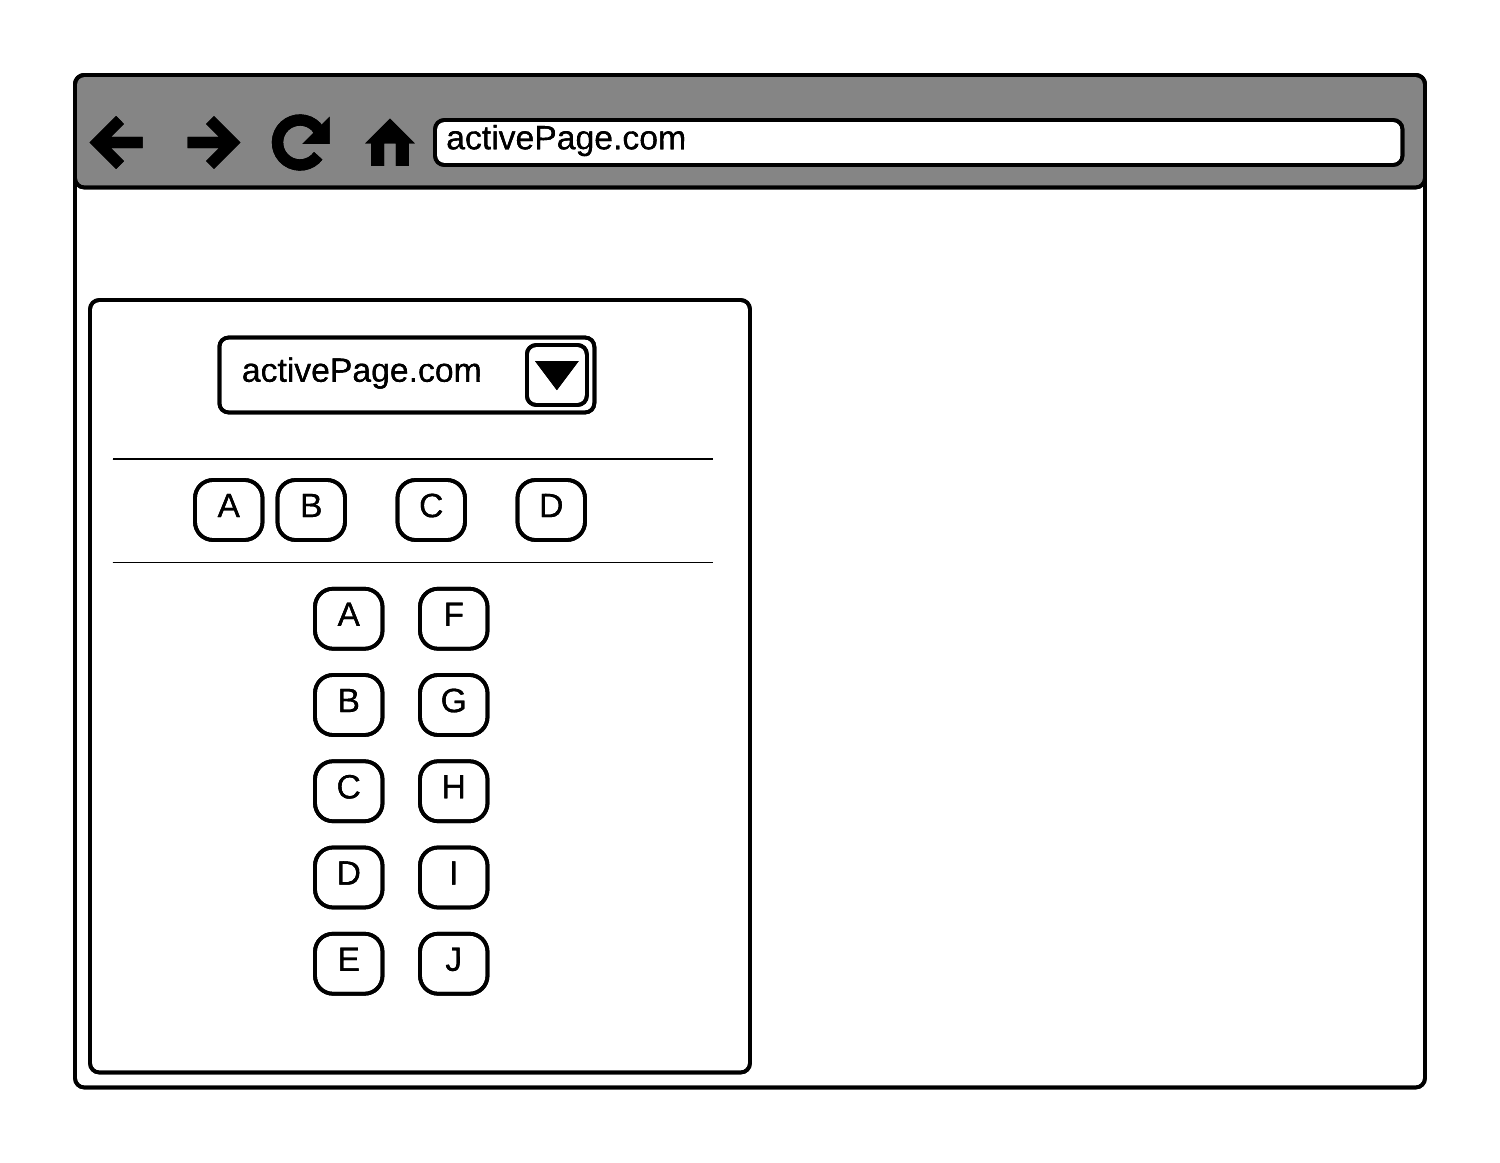
\includegraphics[width=\textwidth]{wireframe2} 
        \caption{Screen seen by the user when loading a site with challenges stored in the system. }
        \label{challenge-screen}
    \end{subfigure}
    \caption{Wireframes illustrating the page schematics of the extension.}
    \label{wireframes}
\end{figure}

\subsection{Implementation}
The implementation follows the design described in the previous section, this section will present how the extension are implemented and demonstrate the actual extension. 


\subsection{Architecture}
\par \autoref{class-diagram} shows the complete architecture of the system.
 The content script attach an event listener to the password field of the active site. If the content of the password field changes, the script sends a message using chrome message passing containing the current length of the password. The controller receives the new password length from the content script, and update the challenges displayed to the user. When the user visits a new site, the url is sent to the controller, which then updates the view with new challenges corresponding to that site.

\begin{figure}[h]
    \centering
    \fbox{ 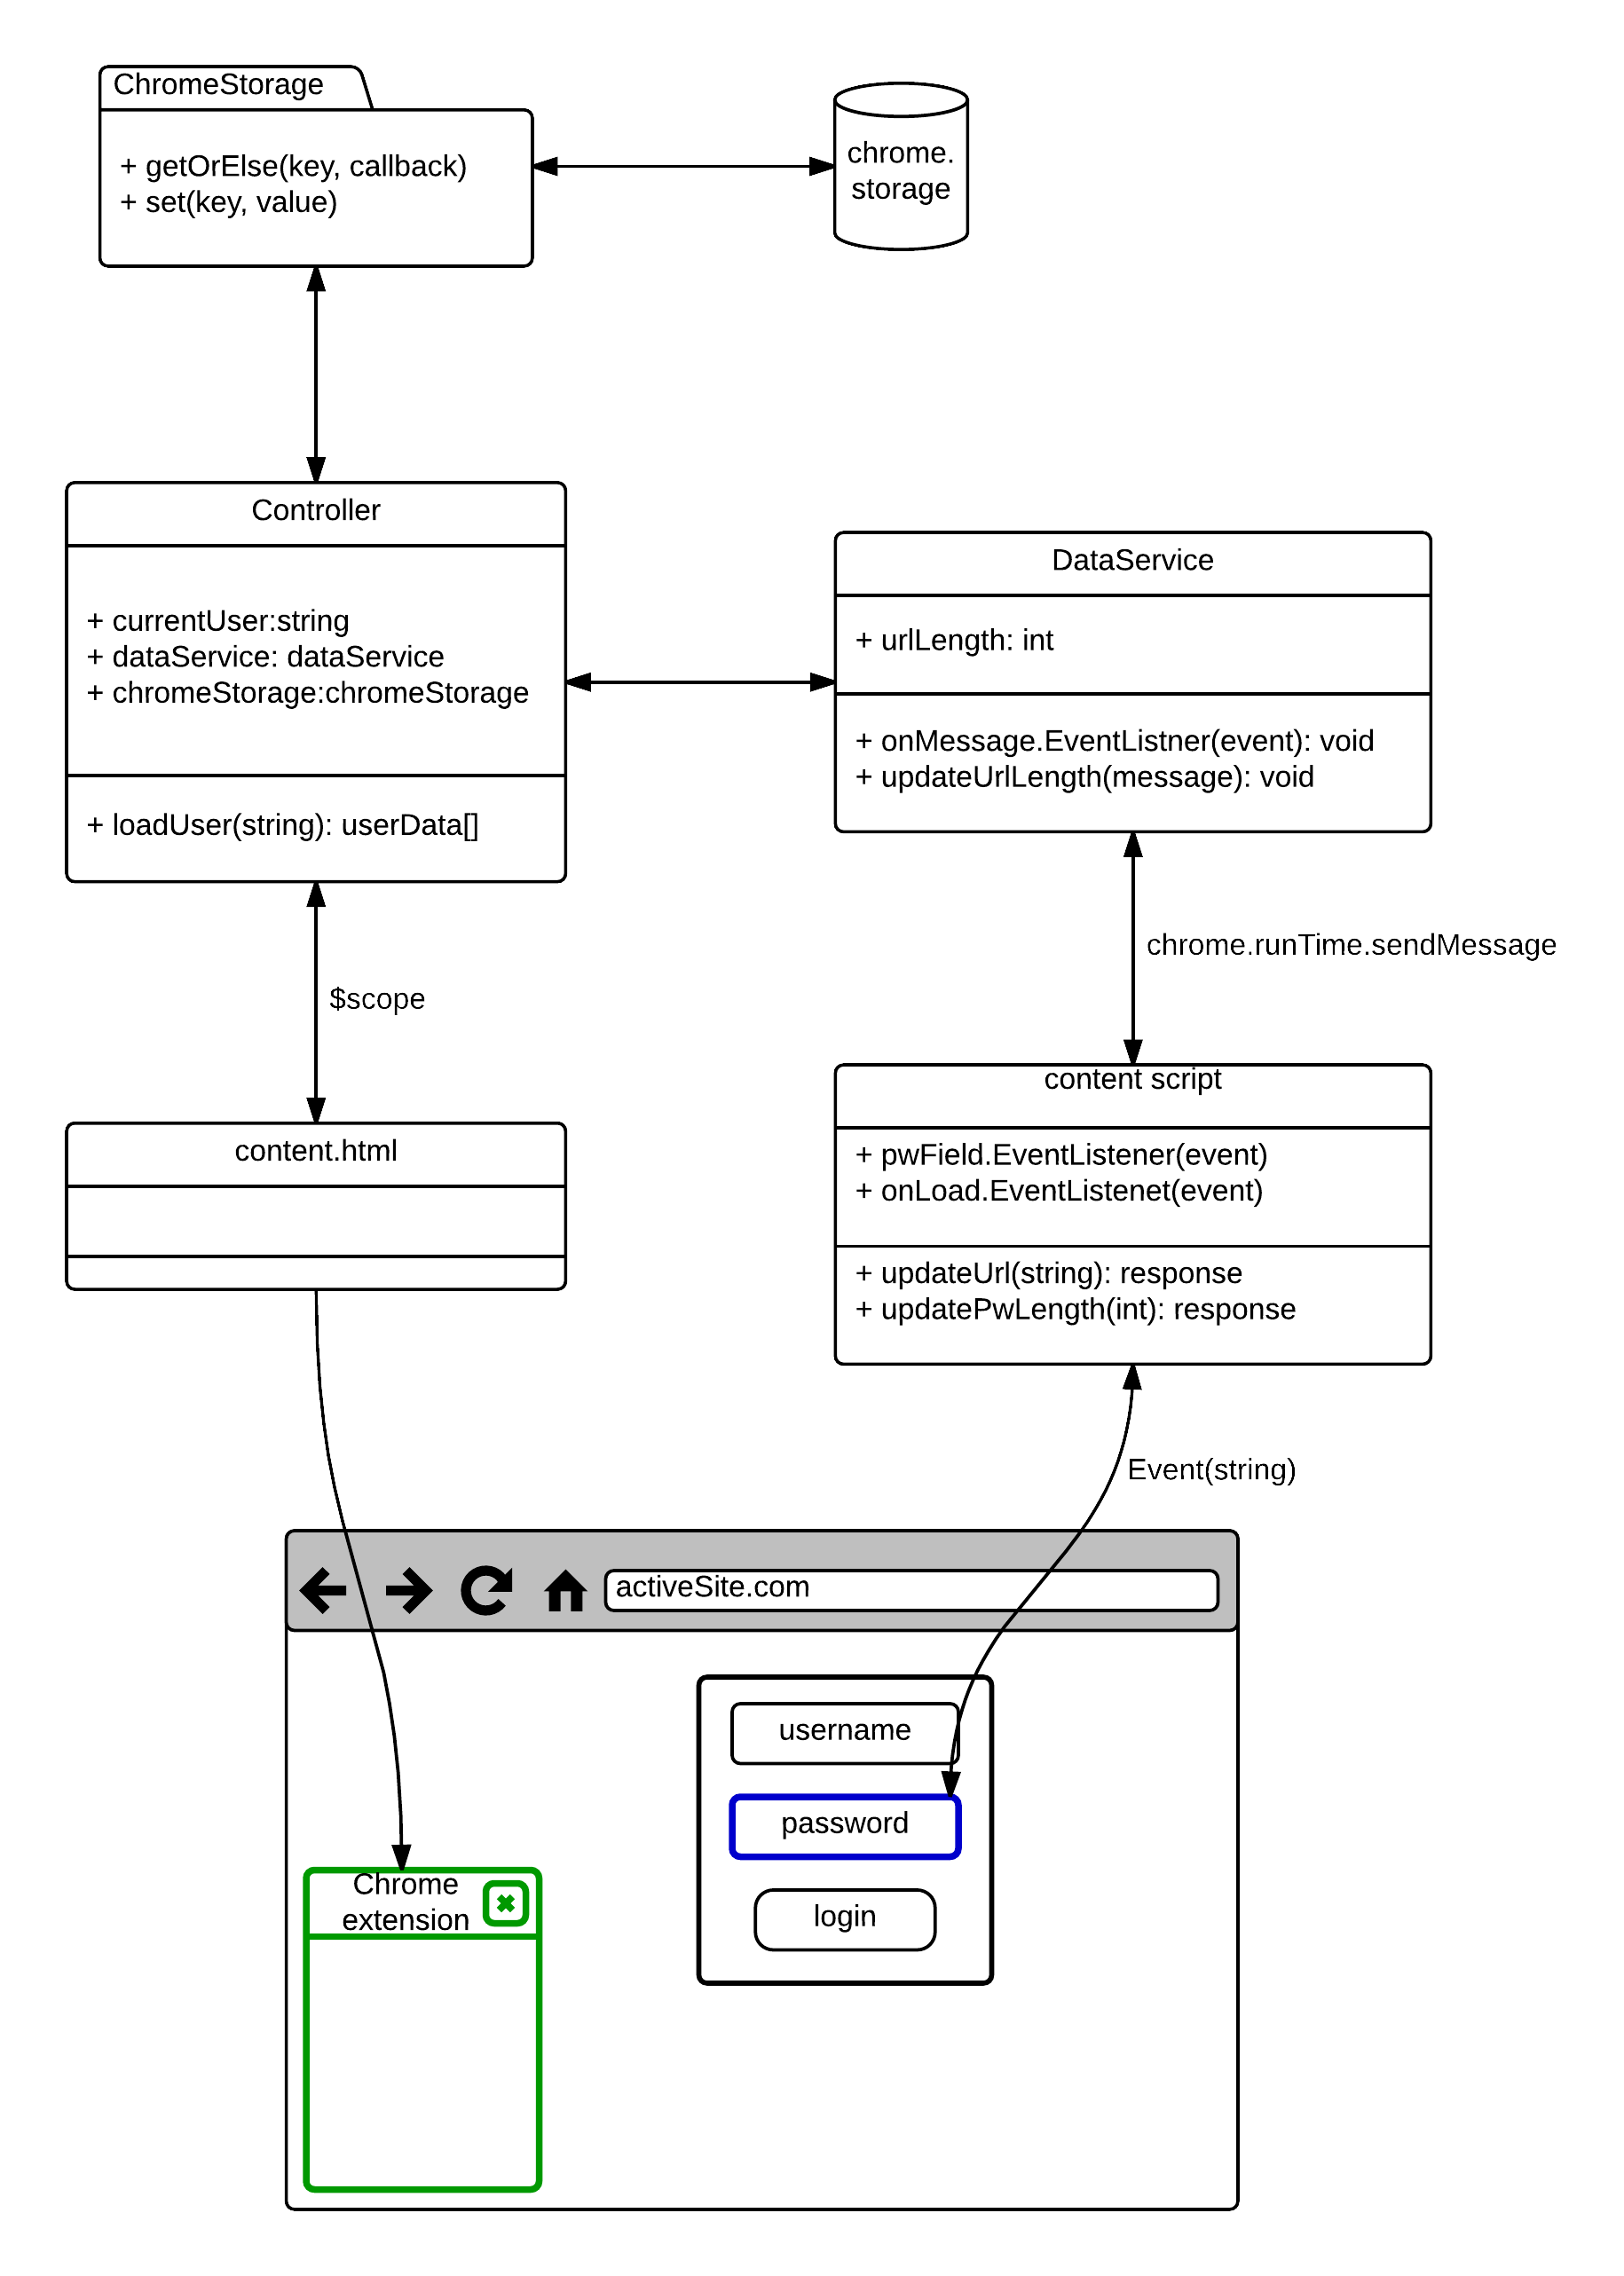
\includegraphics[width=\textwidth]{class-diagram} }
    \caption{Class diagram of the human computable passwords chrome extension.}
    \label{class-diagram}
\end{figure}

\par The classes seen in figure \ref{class-diagram} are all represented in the implemented version of the extension. The construction and responsibilities of the classes are summarized in the following list. The code of the implementation for each component is explained in more detail in appendix \ref{extension-classes}.

\begin{itemize}
    \item \textbf{Controller} is responsible for the business logic related to the information shown to the user in the extension. The controller first tries to load the user data stored in chrome storage, if no user has been created, typically if it is the first time the extension is loaded, a new user is created. The controller keeps track of the url of the current active page and the current length of the password field. It listens for messages from the content scripts and updates the URL and password length variables with the info received. The controller class used in the extension is described in appendix \ref{app:controller}.
    \item \textbf{ChromeStorage\footnote{angular-chrome-storage - \url{https://github.com/infomofo/angular-chrome-storage}}} is a utility resource used to access chrome local storage[\autoref{chrome-storage}]. This module is essentially a wrapper making it easier to retrieve data from chrome storage, while also providing useful debugging and cache management functions.
    \item \textbf{Content script} is responsible for attaching event listeners to the password field of the currently active page.. It also listens to the onload event, sending url updates to the controller every time a new page is loaded. The content script of the extension built in this project can be seen appendix \ref{app:content-script}.
    \item \textbf{main.html} is the view of the application, responsible for the user interface. The view receives updates from the controller through the \$scope variable. When the controller updates in example the current password length, this is reflected in the view where different objects are shown. If the current url is not in the user's list of saved sites, the view will show a dialog allowing the user to add it. When adding a new site the user should update the password of that site using the extension. A snippet of the view is shown in appendix \ref{app:view}. 
    \item \textbf{App.js} is the focal point of the application, responsible for initializing the angular app and routing of views. In this project this file also includes some helper functions which can be seen in appendix \ref{app:app.js}.
\end{itemize}

\paragraph{Launching} the application is done by clicking an icon in the browser toolbar which will launch the extension in a panel floating on top of the other browser windows and tabs. This behavior is specified in the \emph{background page\footnote{Background pages - \url{https://developer.chrome.com/extensions/background_pages}}}. The background page is the "launcher" of the extension, it waits for the user to click the extension icon, firing a browser action event. On catching this event, the script spawns a panel, with the angular application as content. \autoref{background} shows the background page of this extension. After spawning the panel, the background page is standby doing nothing, everything now happens through the angular application running inside the panel. 

\lstinputlisting[caption=Background page., label=background, style=jsStyle, basicstyle=\small, frame=single]{code/background.js}

\subsection{Demonstration}\label{demo}
After launching the extension, as previously explained, the user is presented with the window show in figure \ref{launch-screen}. In this example the active site does not have a record in the user's challenge database, thus the "add new" dialog. By clicking the button, new challenges are generated and stored in the database as a new site. The site is automatically added with the current site domain as key together with randomly generated challenges. Next time the user visits the same page, challenges will appear. After adding a new site, it is the users responsibility to change the password of this site so it matches the challenges.

\par Figures \ref{ch-screens}a-d shows how a user would use the extension when login in to a site. When launching it, the system receive the current sites domain and loads the first challenge corresponding to that site. The user then calculates the first character using the challenges displayed, when this is entered in the password field, new challenges appear until the whole password is calculated. 

\begin{figure}
    \centering
    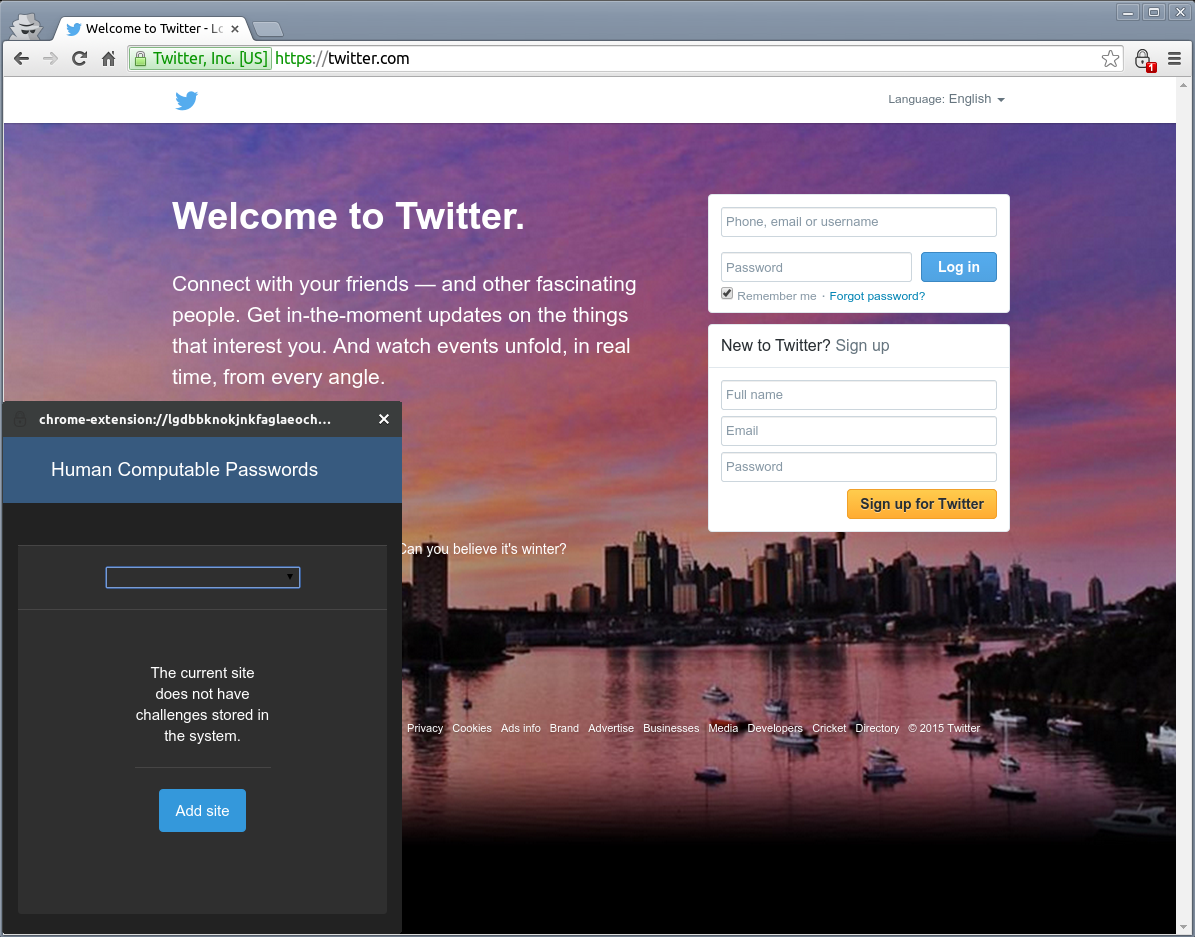
\includegraphics[width=\textwidth]{launch-screen} 
    \caption{Screen as seen by the user after launching the extensions while on a page without stored challenges.}
    \label{launch-screen}
\end{figure}

\begin{figure}
    \centering
    \begin{subfigure}[t]{0.45\textwidth}
        \centering
        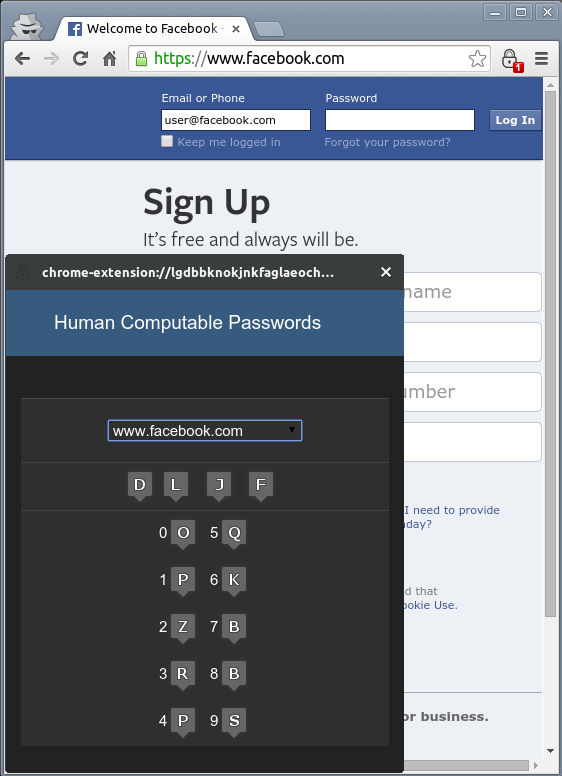
\includegraphics[width=\textwidth]{ch-screen1} 
        \caption{}
        \label{challenge-screen1}
    \end{subfigure}
    \hfill
    \begin{subfigure}[t]{0.45\textwidth}
        \centering
        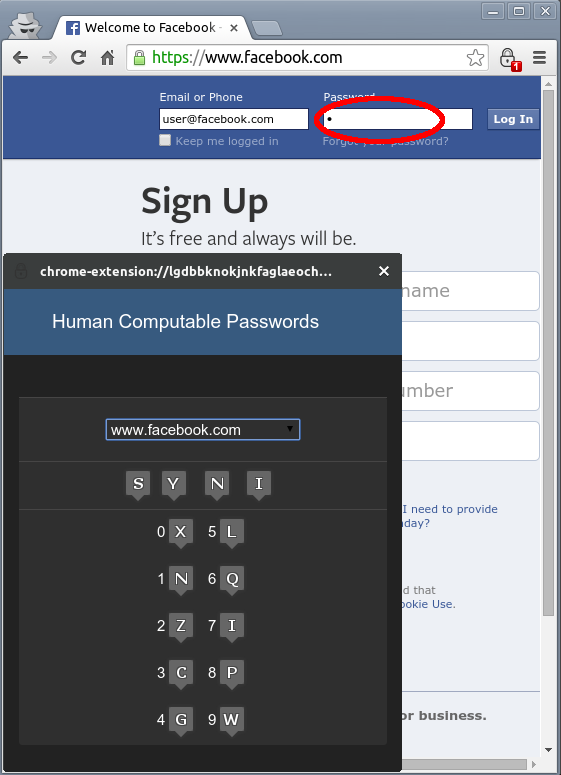
\includegraphics[width=\textwidth]{ch-screen2} 
        \caption{}
        \label{challenge-screen2}
    \end{subfigure}
    \hfill
    \begin{subfigure}[t]{0.45\textwidth}
        \centering
        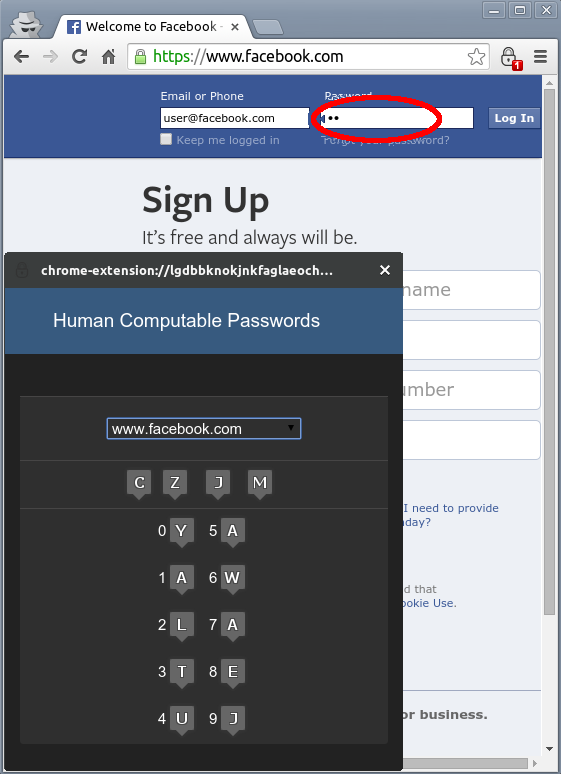
\includegraphics[width=\textwidth]{ch-screen3} 
        \caption{}
        \label{challenge-screen2}
    \end{subfigure}
    \hfill
    \begin{subfigure}[t]{0.45\textwidth}
        \centering
        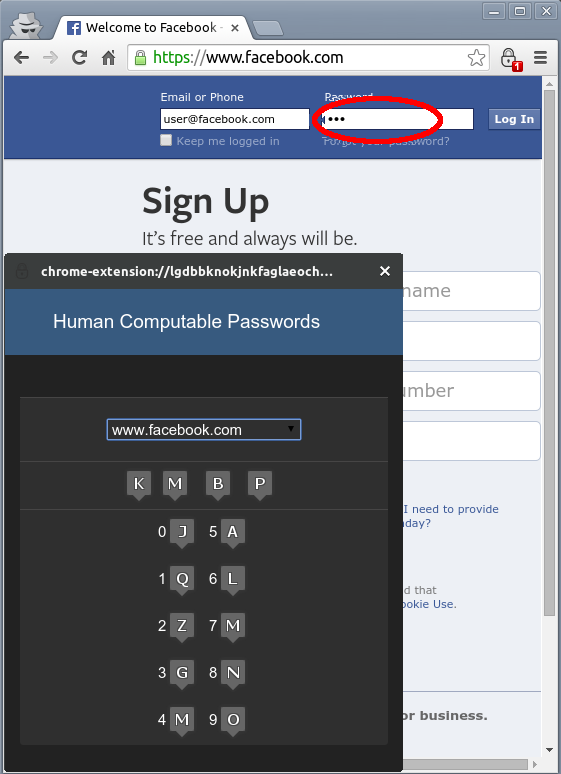
\includegraphics[width=\textwidth]{ch-screen4} 
        \caption{}
        \label{challenge-screen2}
    \end{subfigure}
    \caption{Challenge screens as seen by the user while entering password. The challenges update when the user enter a new character in the password field.}
    \label{ch-screens}
\end{figure}

\newpage

\subsubsection{Data flow}\label{data-flow}
Figure \ref{flow-chart} illustrates the life cycle of the application. When the user visit a site, an event is triggered and caught by the content script, which in turn message the controller about the newly loaded site. The controller then try to load challenges for that site from the storage; if there is a record, the view is updated with the first challenge, if not the "add new"-dialog is loaded. Next event is triggered when the user enters a character in the password field, on receiving notice from the content script the controller updates the view with a new challenge depending on the length of the password. This will then go on until the user has entered the entire password, eventually closing the extension panel.
\begin{figure}
    \centering
    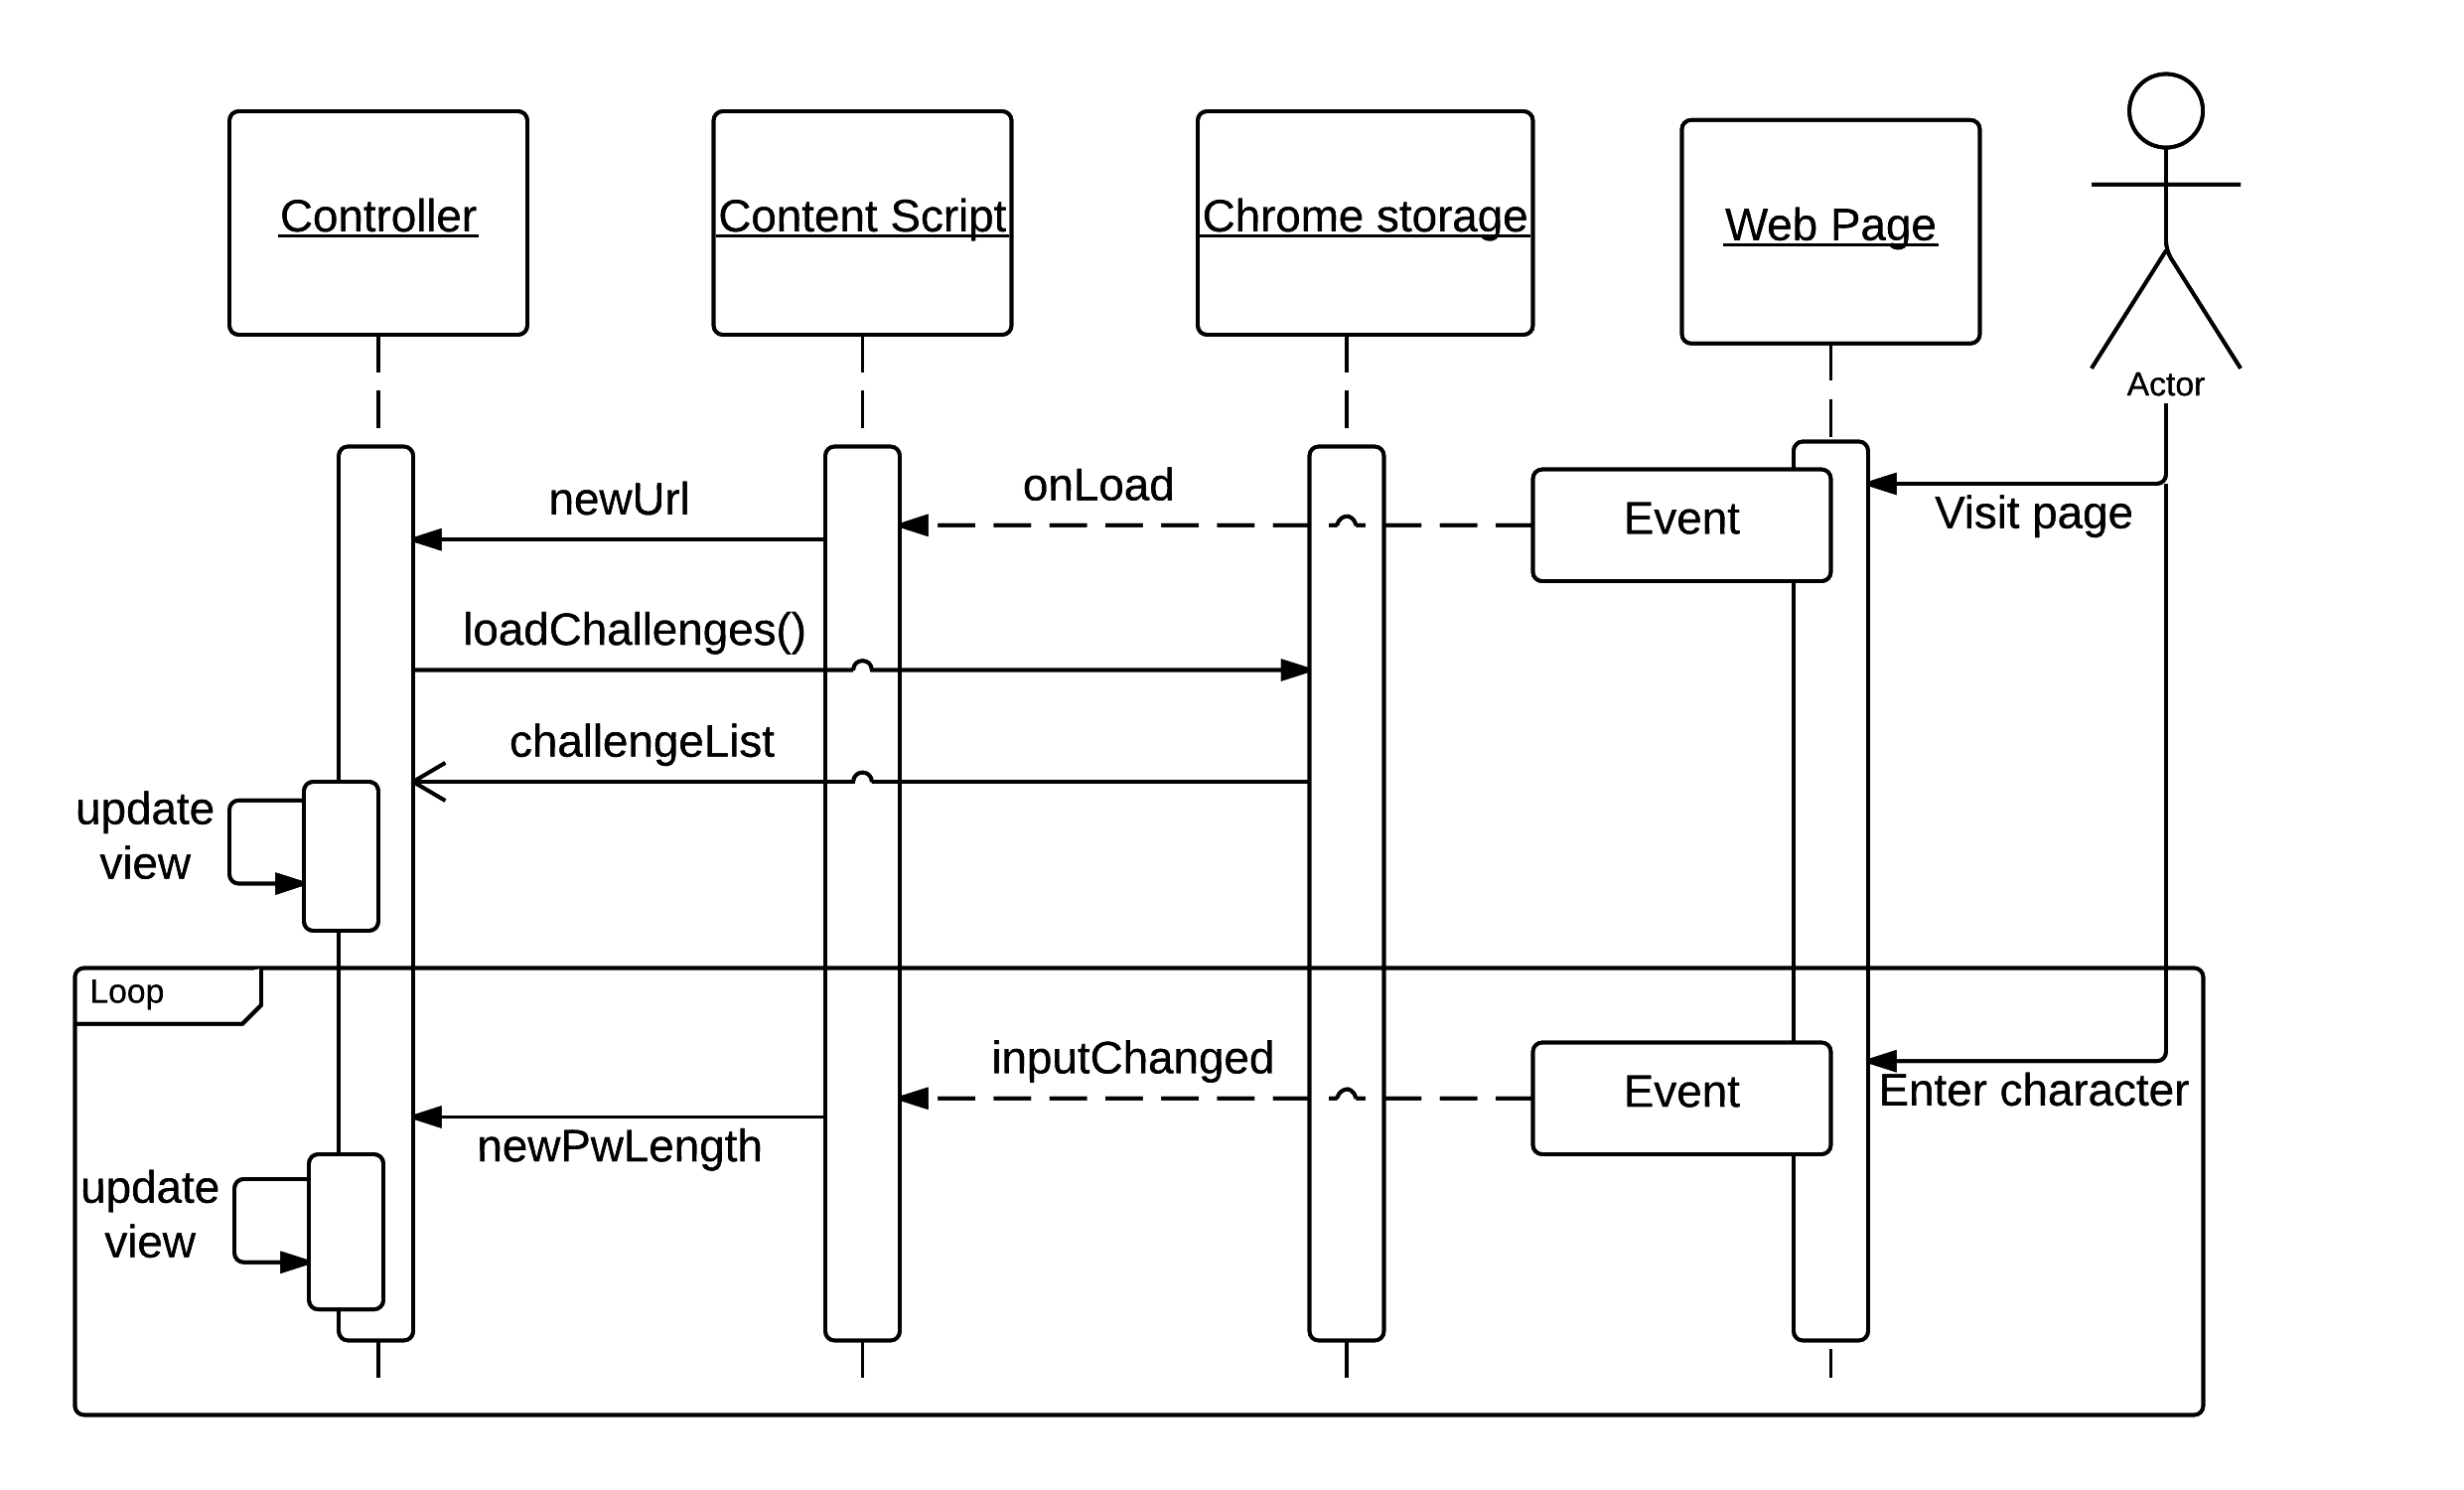
\includegraphics[width=\textwidth]{flow-chart} 
    \caption{Sequence diagram showing the flow in the system when a page is loaded and characters typed in a password field.}
    \label{flow-chart}
\end{figure}

\subsection{Discussion}
The approach of this project when designing the human computable passwords extension was to make an clean and intuitive application making the password management scheme feasible to use. The extension does not require any user interaction, except from when adding new sites, this was done so the user could focus on doing the calculation correctly without having to keep track of the challenges. The scheme itself is also quit complicated so it is important for the user to focus on as few operations as possible. (The simplest approach would be to have a "next"-button for the user to click between every character calculated.)
\par The choice of a browser extension was done with the same mind set, making the application helpful and not distracting. It should be easy to start using the application, requiring as little configuration and managing as possible. The design and construction makes it so that the only real "configuration" required is the changing of passwords when adding sites, which essentially can not be circumvent. Panels is another very useful feature, since the panels floats on top of the other browser windows and keeps in focus while typing. Without panels the user would have to switch between windows when calculating a character and typing it in the password field, which would be a huge drawback both in terms of time and usability. 
\par One apparent problem with using extensions is that they are not supported in mobile browsers, and probably will never be \footnote{Multidevice FAQ - \url{https://developer.chrome.com/multidevice/faq}}. The solution to this would be to make an additional application for mobile, and sync the data to another service available on mobile as well. This could be done quit easily since the data is stored as text, the only change needed would be to substitute the storage module with some other cloud storage service. The problem if the application was built for mobile would be the lack of space to display challenges while typing the password. 
\par The decision to make a browser extension was made on behalf of the mentioned pros and cons, with the most important parameter being disturbance. Only extensions allow a seamless, non-interfering user interface. The other options, namely web application and mobile application, would require switching between windows or at least switching of focus, as well as requiring the user to manually chose the correct site and browse through the different challenges. This is all done automatically with the construction presented in this chapter. The main goal of the design was to include the least amount of unnecessary features, with a clean and unobstructive interface. A summary of the strengths of the chosen design is listed next.

\begin{itemize}
    \item Easy to use, require less to no user interaction after configuration.
    \item Panel that stay on top while entering the password allows for quick and easy calculation without stopping to update and manage challenges.
    \item Chrome.storage.sync automatically synchronize the stored challenges to the users google account allowing persistent usage across devices and accounts.
    \item All data is stored as text strings, this makes it easy to integrate with other services in the future. The user could also store the challenges elsewhere if need be, e.g. as text locally or even print the challenges on paper in the extreme case.
\end{itemize}








\chapter{Usability Experiment}\label{ch:experiment}
This chapter presents the design and execution of an experiment trying to measure  the performance of the HCP scheme. The experiment is designed as a web application implementing the scheme, allowing participants to test how the scheme would work in practice while measuring how fast and reliable the computation is performed. The application acts as both a demonstration app and a tool for gathering performance data. It has four sections designed to help the participants understand the scheme and get familiar with the computation technique. First, a demonstration video is shown explaining how to compute a password from a challenge, then users are asked to enter some demographic data. Next is the practice section, where users are supposed to practice doing the calculation until feeling comfortable solving challenges without error. Finally is the experiment part, where the calculations are timed and correctness monitored. After finishing the calculations user submit the data and can choose to continue doing more experiments now, or later.
\section{Experiment Objective}
The goal of the experiment is to measure how hard it is for a user to learn the scheme, i.e. how fast and reliable users do the calculations. The experiment measures the calculation times of the participants, and also monitor their progression after several trials. Users should also be able to calculate passwords without too many mistakes. The failure rate is maybe the most important variable to measure; if a user averages more than one mistake for each password calculated the scheme would not work in practice, since most passwords calculated would be wrong. 
\par It is important to note that this project does not see the HCP scheme as a replacement for the widely used standard password managers. It is regarded as a solution for users interested in a secure and reliable way of keeping track of strong passwords, without having to trust a password management service or application. This experiment tests if it is even possible, for users willing to go through the trouble of learning a secret mapping, to use the scheme as an everyday solution.

\par The objectives of the experiment can be summarized as the following.
\begin{itemize}
    \item Measure the average calculation times, both for each participant and for the whole population.
    \item Measure how much users improve after several trials.
    \item Measure the average failure rate for each participant.
\end{itemize}


\section{Method}
The experiment does not try to test any preset hypothesis as it is not clear what to expect regarding either of the tested values. It is not known how hard it is do to the calculations, neither regarding calculation times or failure rates. The results of the experiment does not give an answer, but rather a basis for further data collection through larger scale experiments, for example using crowd sourcing or social medias.

\par Exploratory data analysis (EDA) was introduced by John W. Turkey~\cite{turkey} and involves analysis of data without a prior hypothesis to test. The technique promotes exploration of data to possible find characteristics not previously considered, and essentially suggesting hypotheses to be tested in later surveys or experiments. Velleman and Hoaglin~\cite{exploratory-analysis} describe EDA as a contrast to the formal scientific method involving stating a hypothesis, collecting data and applying a statistical test of the hypothesis. EDA often involves making graphical representations of the data, and then trying to find interesting characteristics and relations. EDA does not conclude with a hypothesis test based on the collected data, but is the first step of an iterative process trying to reveal facts. 

\begin{remark}
 The project does not store any personal information about the participants, and is thus not subject to notification to the "Norwegian Social Science Data Service"\footnote{Is my research project subject to notification? - \url{http://www.nsd.uib.no/nsd/english/pvo.html}}. The experiment only records an anonymous id plus the experiment results consisting of computation time and correctness of the calculations done. Some demographic data is also recorded (age, area of study), but the data can not be connected to person and are thus not regarded as personal information.
 \end{remark}

\par After conducting the experiment, the data is examined and significant characteristics discussed. There are some obvious parameters to explore, including means and standard deviation of the calculation times and failure rate, as well as how these change with practice. 

\par The usability of the scheme directly relies on the calculation time and failure rate as discussed in section \ref{sec:usability}. This can be discussed further after obtaining some numbers giving a picture of what is normal and possible in terms of speed and reliability.


\par A result showing that more than 95\% of all calculations are correct would be promising, since it would mean that approximately 60\% of the passwords calculated would be correct, given length 10 passwords. If the failure rate is significantly worse, the scheme would more often than not be useless since most users would obtain a faulty password when trying to log in. The conclusion of the experiment presented in this project will either way have to be tested more thoroughly, possibly using the same experiment setup or preferably with a throughly random mapping as well. 



\section{Experiment Setup}
The experiment presents and demonstrates the calculation technique to the users, which then is given a chance to practice until fairly familiar with the mechanics. Finally users are asked to calculate a complete password challenge, from which the time spent on each single digit challenge is recorded, as well as if the calculation was correct or not. The practice section allows users to learn through trial and error, using backspace to go back and forth between challenges while also given feedback on the correctness. The experiment view on the other hand does not give any feedback and does not allow user to go back after entering a character. This is done to make sure all mistakes are recorded, even if it is only a miss click. 
\subsection{Secret Mapping} The biggest decision made in regards to the experiment design was how to simulate the operation ``recall'' i.e. recalling from memory. It would not be feasible to ask all the participants to memorize a secret mapping beforehand as this would make it very hard to find volunteers. The chosen solution to this problem is to include a ``cheat sheet'' in addition to the displayed challenges, i.e. a list of object to digit mappings shown separately but in the same view as the challenge.
\par After some testing it became apparent that there was a big difference between recalling from memory and actually ``reading'' from a list, which this approach eventually is. To make the operation more similar to the desired recall operation, the mapping was changed from random alphabet positions (e.g A=1, B=2, C=3). This way one does not always have to read in the table to know the mapping. Most users will be able to know instantly what the mapping for at least the first and eventually, after some practice, all the letters, much easier than with a random mapping. The is the closest way of mimicking the actual operations of the scheme without having the participants memorize an actual mapping. It is not in any way certain that this shortcut reflect the real world act of recalling from memory, but it is assumed to be ``close enough'' for the experiment. 
\begin{remark}
The author of this project did memorize a mapping of both 10 and later 20 mappings without significantly different calculation times compared to using the alphabet positions.
\end{remark}

\subsection{Participants}
The participants for the experiment were chosen mostly from people known by the author, this limits the number of participants somewhat. This was done to ensure the quality of the data samples. The experiment could have been distributed through crowd sourcing services or social media, probably increasing the number of participants drastically. The problem with this approach, and the reason for not doing it, is that the experiment requires absolute concentration which can not be assured from ``casual'' participants accessing the experiment through a link posted on facebook. Since every participant calculates 10 single digit challenges for each trial of the experiment, there is still a decent amount of data samples, even with relatively few participants. 
\par Even if the experiment might be limited by the number of participants, the results are still considered to be interesting. Since the scheme tested is not supposed to be a widely-deployed password manager, it might be sufficient if the experiment can show that some users are able achieve what is considered sufficient usability. It should also be noted that most of the participants are regarded above average in mathematics. This might be a strength or a weakness of the experiment as it does not represent a wide range of the population, but the calculation times should at least be stronger than average.


\section{Web Application}
The experiment application is similar in design to the Chrome extension presented in \autoref{app}, but implemented as a web application. It is implemented using the AngularJS framework (as described in \autoref{app}) and a mongoDB\footnote{mongoDB - \url{https://www.mongodb.org/}} database to store the results, a cookie in the users' browser is used to keep track of users across trials. 

\par The application consists of four sections to flip through, with the last one being the actual experiment. First, users are presented with a video demonstration of the scheme and instructions on how to calculate passwords. The slides used to instruct users can be seen in \autoref{demo-slides}. After watching the demo, users are asked to enter some demographic data (age and occupation). Next, is a section which looks the same as the experiment, but without the actual recording of data, this is the practice section. The purpose of this section is to give users a chance to verify that they have understood the scheme and are actually able to calculate passwords. When users are ready to start the experiment, they can continue on to the actual experiment, which is the final view. The experiment is exactly like the practice section, without response on correctness and redo capabilities, with backspace deactivated. The first sample of the experiment is not counted towards the results, allowing users to get ready and start when they feel like it. 


\par Section \ref{computation-time} discusses how a single digit challenge can be presented to users in a logical way, possibly making it more efficient to calculate. The experiment uses a similar layout to the one shown in \autoref{challenges} and also as in the Chrome extension in chapter \ref{app}. The challenges update in the same way as in the chrome extension so users should be able to calculate the responses continuously. The calculation time is recorded for each single digit challenge computed, together with a boolean value representing if the result was correct or not. 
\par Figure \ref{complete-experiment} shows the screen after completing a trial of the experiment, next users will push the submit button and the sample would be saved in the database together with a random identification stored in a cookie in the users' browsers. Users can then redo the experiment several times keeping the same id, making it possible to track each participant's development.

\begin{figure}[h]
    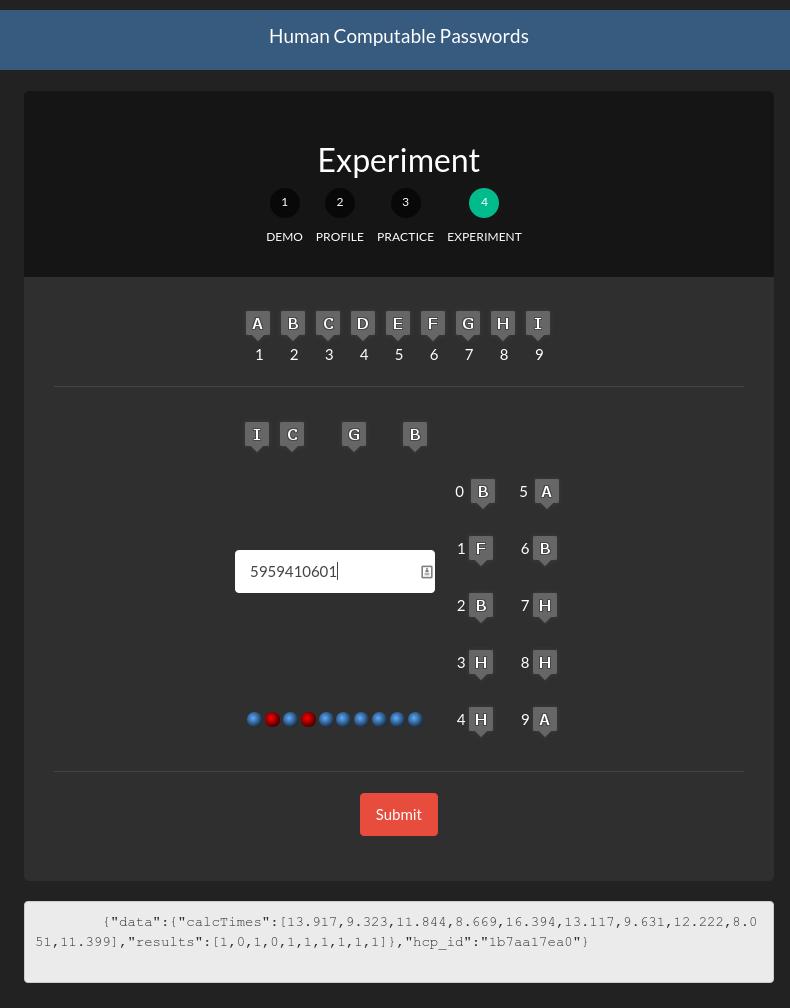
\includegraphics[width=\textwidth]{complete-experiment}
    \caption{The experiment screen seen after completing an experiment sample, ready to be submitted.}
    \label{complete-experiment}
\end{figure}

\par As for the storage of results a noSQL database called MongoDB is used. After completing a trial of the experiment a Javascript object is stored in the database, \autoref{db-obj} shows an example of this object. Note the \emph{hcp\_id} field which is fetched from a cookie in the participants' browsers, making it persist across several trials. 

\par The views of the web application can be seen in \autoref{experiment-views} or by visiting the hosted experiment site at \url{hcp.sp1nakr.com}.

\begin{table}
\begin{tabular}{|c|c|}
    \hline
    hcp\_id & 1b7aa17ea0  \\ \hline
    occupation & Technology student \\ \hline
    age & 27 \\ \hline
    results & $[1,1,1,1,1,1,1,1,1,1]$ \\ \hline
    calcTimes & $[12.047,7.115,8.022,9.283,10.544,8.807,9.925,9.78,7.11,8.187]$ \\ \hline
\end{tabular}
\caption{Experiment object after completing a trial, as stored in the database.}
\label{db-obj}
\end{table}

\section{Results}

This section presents the results of the conducted experiment and investigate the characteristics of the data recorded. The focus is on the calculation times and failure rates, which both are important factors in the resulting usability of the scheme, as discussed in \autoref{sec:usability}.
\par The observations made are not necessarily representative for all users, because of the relatively small number of samples ($467$ single digit challenges), but it is still interesting to investigate the consequences of the results. Even if the results show that the scheme achieves a lower level of usability than what are considered acceptable, it might still function well for some users with the right amount of practice. The limitations of the experiment is discussed, in addition to results and the consequences of these.

\subsection{Calculation Times.}
How fast a user is able to calculate the response to a single digit challenge is a concrete measure of the usability of the scheme. Figure \ref{histo-calctimes} shows the distribution of calculation times of all the experiment samples, the calculated average off all the $467$ trials are $10.296$ seconds. The median value is $9.406$ with standard deviation of $3.64$ which also can be observed in the figure. 
\par Recall conjecture \ref{conjecture1} from \autoref{human-func}. The function $f$ (see definition \ref{fo-function}) used in this project is $(P,9,3)$-computable. The conjecture then defines the variable $\gamma_H$ for user $H$ as {\Large $\gamma_H = \frac{\hat t}{9}$}. 
\par The average $\gamma$ of all the participants are $\tilde \gamma = \frac{10.104}{9} = 1.227$. This is slightly higher than the $7.5$ seconds ($\gamma_H \le 1 $) Blocki~\cite{hcp-blocki} predicts that users with moderate mathematical backgrounds should achieve. It is still not unreasonably high, and should not be a direct hindrance. Calculating a 10 character password would for example take $10 \cdot 10 = 100$ seconds, just above $1.5$ minutes, to calculate, 15 character would take $2.5$ minutes. On average spending 2-3 minutes calculating a password might seem like a lot, but users concerned about the security of their accounts, might be willing to make this trade-off. Especially if users are worried about putting passwords in the hands of a online service to store persistently (e.g. \emph{lastpass.com}), might be willing to put quite some time into calculating passwords instead.
\par It is also relevant to study the evolution of each user in terms calculation times. Figure \ref{scatter-regression} illustrates the average calculation time for each $i$th trail per user. $i=1$ represent the average of the first calculation done by each user, $i=2$ the second calculation etc. The figure clearly illustrates that the averages decrease with practice. This could have been expected, since users will be more and more familiar with the calculation procedure for each trial. The consequence of this observation is that the average calculation time, and consequently $\gamma$, would be significantly lower if the participants got more practice with the scheme before their results was recorded. Each participant averaged $33$ samples each, so it is not feasible to e.g. calculate the average after removing the 20 first calculations from each participant, as this would leave very few trials. The important goal of the experiment is though not to find an accurate average calculation time, but to verify that $\gamma_H \le 1$ is achievable. It seems that the average most likely is somewhere between 9 and 11 seconds, depending on how long users have been using the scheme, which is not severely limiting.
\par Figure \ref{user-regression} and table \ref{tbl:bestuser} shows the 7 participants with the most samples, the same effect can be observed, all except from one participant have a downward going trend (see SCT in table \ref{tbl:bestuser}).

\begin{table}[h]
    \centering
\begin{tabular}{|c|c|c|c|c|}
    \hline
     SMP & MCT & SDCT & SCT & MFR \\ \hline \hline
    $72$ & $9.02$ & $2.38$ & $-0.015$ & $0.0695$\\\hline
    $36$ & $10.06$ & $3.24$ & $0.038$ & $0.1944$\\\hline
    $72$ & $9.62$ & $2.79$ & $-0.373$ & $0.0278$\\\hline
    $45$ & $10.33$ & $3.33$ & $-0.115$ & $0.044$\\\hline
    $45$ & $10.06$ & $3.31$ & $-0.068$ & $0.089$\\\hline
    $36$ & $9.89$ & $3.34$ & $-0.143$ & $0.083$\\\hline
    $45$ & $9.88$ & $3.33$ & $-0.023$ & $0.022$\\\hline

\end{tabular}
\caption{Table of the 7 best participants. SMP=sample size, MCT=mean calculation time, SDCT=standard deviation of calculation time, SCT=slope calculation time, MFR=mean failure rate. }
\label{tbl:bestuser}
\end{table}


\begin{figure}
    \centering
    \begin{tikzpicture}
        \begin{axis}[width=\textwidth, xlabel=Calculation times in seconds. ,ybar, ymin=0, ylabel=Number of single digit challenges.]
            \addplot +[
                    hist = {
                        bins=25,
                        data min=3,
                        data max=20
                    },
                    fill=blue!60
                ]table [y index=0]{calcTimes2.csv};

        \end{axis}
    \end{tikzpicture}
    \caption{Histogram showing the distribution of calculation times of all the recorded experiments. Sample size $467$ single digit challenges.}
    \label{histo-calctimes}
\end{figure}


\begin{figure}
    \centering
\begin{tikzpicture}
    \begin{axis}[
                enlargelimits=false,
                xlabel=Trial number: $i$,
                ylabel = Average calculation time in seconds.,
                width=\textwidth,
                ymin=4,
                ymax=18
        ]
        \addplot+[
                only marks,
                scatter,
                mark size=1.5pt
            ]
            table[meta=avg]
            {sum-avgs2.dat};
        \addplot[
            domain=0:80,
            samples=3,
            very thick
        ]{11.42687437-0.05270738*x};
    \end{axis}

\end{tikzpicture}
\caption{Average calculation time of all participants' $i'th$ calculation sample, and the regression line of the averages. Sample size $467$, average samples per participant $33$.}
\label{scatter-regression}
\end{figure}


\begin{figure}
    \centering
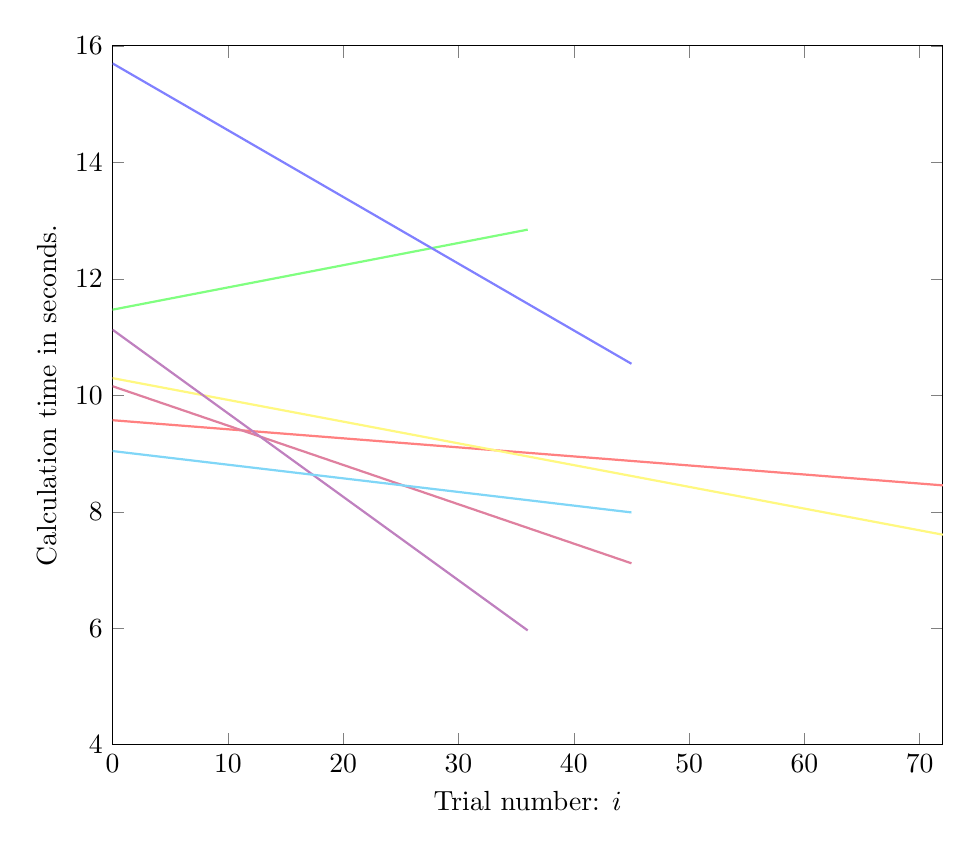
\begin{tikzpicture}
    \begin{axis}[
                enlargelimits=false,
                xlabel=Trial number: $i$,
                ylabel = Calculation time in seconds.,
                width=\textwidth,
                ymin=4,
                ymax=16
        ]
        \addplot[
            domain=0:72,
            samples=3,
            thick,
            color=red!50
        ]{9.572-0.015535*x};
        \addplot[
            domain=0:36,
            samples=3,
            thick,
            color=green!50
        ]{11.46978+0.03817*x};
        \addplot[
            domain=0:72,
            samples=3,
            thick,
            color=yellow!50
        ]{10.29454-0.037335*x};
        \addplot[
            domain=0:45,
            samples=3,
            thick,
            color=blue!50
        ]{15.6977-0.1146*x};
        \addplot[
            domain=0:45,
            samples=3,
            thick,
            color=purple!50
        ]{10.15532-0.06755*x};
        \addplot[
            domain=0:36,
            samples=3,
            thick,
            color=violet!50
        ]{11.12582-0.143408*x};
        \addplot[
            domain=0:45,
            samples=3,
            thick,
            color=cyan!50
        ]{9.04245-0.023411*x};
    \end{axis}

\end{tikzpicture}
\caption{Regression lines for the 7 participants with the most samples. A clear downward sloping trend in terms of calculation time is observed.}
\label{user-regression}
\end{figure}



\subsection{Failure Rate.}
Failure rate is a key characteristic of the scheme. As mentioned it is essential that a user is able to calculate passwords correctly for the scheme to function. How high the failure rate can be depends on how long passwords are used and how often a user can enter the wrong password without locking the account. A typical password protected site will allow a minimum of three strikes before the account is locked~\cite{10-strikes}. It is thus important that the probability of being ``locked out'' is small enough for it not to happen often, how often is of course subject to discussion.

\begin{observation}\label{obs:failrate}
    Average failure rate for all samples recorded in the experiment was measured to be $\tilde \lambda = 0.0584795321637$, approximately every one out of 17 single digit challenge was calculated wrong.
\end{observation}
This observation might not seem very unusual, but since a password consists of a sequence of calculations, it is required that users calculate a given number of challenges consecutively without failure. It is thus more interesting to evaluate the probability of having at least one mistake in a complete password calculation sequence. It is also not unusual to enforce a password policy using a three-strike policy which locks the account if three consecutive mistakes are made. Next, these probabilities are presented and discussed. 


The probability of having at least one mistake in a length $l$ password given the failure rate $\lambda$ is given by
\begin{equation}\label{eq:failrate}
    P(fail) = 1 - (1 - \lambda)^l
\end{equation}

Next, the probability of getting the account locked given a three-strike policy with the same password and failure rate is 
\begin{equation}\label{eq:lockrate}
    P(lock) = ( 1 - (1 - \lambda)^l )^3
\end{equation}


\begin{table}[h]
    \centering
\begin{tabular}{|c|c|c|c|c|}
    \hline
    Password length $l$ & $3$ & $5$ & $10$ & $15$ \\ \hline \hline
    $P(fail)$ & $0.1654$ & $0.2601$ & $0.4526$ & $0.5959$ \\ \hline
    $P(lock)$ & $0.0045$ & $0.0176$ & $0.0927$ & $0.2107$ \\ \hline
\end{tabular}
\caption{Probability of having at least one mistake in a length $l$ password given failure rate $\lambda = 0.0584795321637$ for each single digit challenge.}
\label{tbl:failrate}
\end{table}
 
\par Observation \ref{tbl:failrate} shows the probabilities of calculating a password wrong once and three times in a row. If users want to use a password of 15 characters, which is reasonable to assume since the scheme only produce digits, they will compute a faulty password nearly 60\% of the time. This limits the usability severely, since users will more often than not, be unable to log in.
\par The probability of actually locking the account by miscalculating three passwords in a row, is lower but not significantly. With the same failure rate and password length, users would break the three-strike rule approximately one out of five login attempts.

\par To illustrate this consequence in a extreme case, consider the \emph{very active} user from table \ref{users} in section \ref{sec:usability} who visits 10 different accounts every day. Such an user would eventually lock two accounts every day with password lengths of 15 characters, which of course is not acceptable.

\par As discussed in \autoref{improving-usab} (and as implemented in \autoref{app}), the password length needed for different accounts may vary. By using shorter password for noncritical accounts, and only generating long passwords for the most critical, the average password length will be much lower than in the examples above. The scheme could then be tweaked by users to fit specific needs, instead of requiring 10 or 15 characters in all passwords generated. For less sensitive accounts users may have passwords of lengths 5, which would make for a mistake in approximately every 4th password, and only locking an account every 57th login attempt. This way users can calculate passwords with significantly less effort and lower failure rates. 

\par The experiment did not find any significant correlation between failure rates and calculation times. Users calculating fast do not have a higher failure rate than slower users, which some might expected. 

%\subsection{Improvement Measures.}
%\par Blocki et al.~\cite{hcp-blocki} suggests a tweak to the scheme with the purpose of decreasing the calculation time while still ensuring resistance against dictionary attacks. The suggestion is to memorize another mapping $w:\mathbb{Z}_{10} \rightarrow \{x\}$ with $x$ being one of the $10000$ most common English words. Then after computing $f(\sigma(C))$ the user would apply $w$ giving the corresponding word to the digit. The point of doing this is to save time when calculating, but it also solves the problem with high failure rates. Blocki argues, it would be sufficient with 3-5 challenges. With this assumption that 3-5 calculations are enough, the scheme would function significantly better. 
%\par Using the same example with the very active user, an account would be locked every 222nd login attempt with length 3 and every 57th with length 5. This would be a huge improvement, actually making the scheme usable.


\begin{remark}
    The author remarks that the findings related to failure rates might be too harsh since the participants was asked to calculate the challenges ``as fast as possible'', which might be the wrong approach. In a real world scenario it would be more important to calculate correctly. Though, the results clearly show that the failure rate is a relevant attribute worth investigating closer, as it might limit the reliability of the scheme in real usecases.
\end{remark}





\chapter{Concluding Remarks and Further Work}
This project has presented the human computable password management scheme by Blocki et al.~\cite{hcp-blocki}, as well as the design and construction of two applications implementing the scheme with different purposes. How different characteristic and parameters affect the usability of the scheme was discussed, as well as how password length and number of secret mappings affect the security. Failure rate was introduced as a important factor affecting the usability of the scheme. 
\par The first application is a Google Chrome browser extension, making it easy for users to employ the scheme without too much trouble. It is a fact that the scheme is quite complex and require a lot dedication from the user for it to work. It is thus important to have a tool minimizing extra work required, including management and generation of challenges. Without a tool to take care of these obstacles, the scheme would be very hard to use in practice. With the application created in this project, a user only have to worry about memorizing and rehearsing the secret mapping, all the overhead related to generation, storing and fetching of challenges is handled by the extension. The one choice the user have to make is what category to put the site in, either low, medium or high sensitivity. This measure was introduced to increase the usability by lowering the average number of single digit challenges, while still keeping the important accounts secured.
\par The application is available in the browser, making it very accessible in situations where passwords are needed. The extension monitors the active page browsed by the user and fetches information from DOM allowing it to display the correct challenge at all times, both in regards to which page the user is visiting and how many characters are entered in the password field. E.g. if the user visit google.com the extension will get notice about this and bring up the challenges associated with google.com, if the site is note part of the system, the user will get the chance to add it. When calculating passwords, the challenge on display update for each entered character in the password field.
\par The second application is a web application functioning as a demonstration platform as well as a experiment, gathering usage data. The experiment gathers data related to calculation time and failure rates. It was created to investigate how the scheme performs, with usability characteristics in focus. The participants in the experiment, gets a short introduction and the chance to practice until fairly familiar with the scheme. And are then asked to calculate a complete password consisting of 10 singlet digit challenges, while getting timed.
\par The experiment measured a average calculation time of $10.922$ seconds, with a standard deviation of $3.64$. This is considered to be reasonably good, as it should not limit the usability of the scheme severely. It could also be observed that users improved over time so that average calculation time would probably be even lower after some practice. 
\par A more unanticipated result was the failure rate, which was measured to be $0.058$, meaning that every 17 single digit challenge would be calculated wrong. This result should not be interpreted as a dismissal of the scheme, since different users will achieve different failure rates, and many will be able to calculate correctly most of the time. What should be emphasized though, is that the failure rate should be investigated closer, to verify that a general user average a low enough failure rate. 


\section{Further Work}

\subsection{Additional Applications.}
This project showed how browser extensions can be used to create an easy to used password management application. This choice was made with a goal of making a quite complex scheme usable without too much overhead and practice. To make the scheme even more accessible, it would be by creating an accompanying web application and possibly a mobile application. These applications could use the same storage, while still syncing the to chrome storage for the browser extension and to mobile storage for the mobile application. It would be useful to have a user management page to overview user data and challenges. The construction presented here does not allow the user to manually configure the account which some users might dislike. 

\subsection{Larger scale experiments}
It is, as mentioned, clear that the failure rate of the scheme is important for it to function in practice. The experiment conducted in this project did not aim to tell a truth or verify a hypothesis, which should be the next step. A typical setup would could be similar to the one presented here, but in a much larger scale, possibly using a crowd sourcing service or social medias, asking the participants to calculate challenges. It would be important to get more samples from each participant, making it easier to calculate different averages after more practice.  
\par It would also be interesting to conduct a survey gathering data about how users rate their account. Typically asking how many they regard as "highly sensitive", "don't-care" etc. This would make it possible calculate an average password length which again could be used to measure failure rates and calculation times more thorough. 

\renewcommand*{\bibname}{References}
\bibliographystyle{alpha}
\bibliography{main,biblo}







\appendix
\addtocontents{toc}{%
 \protect\vspace{1em}% 
 \protect\noindent \bfseries \appendixtocname\protect\par
 \protect\vspace{-.5em}%
}
\renewcommand{\chaptername}{\appendixname}

\chapter{Demonstration slides}

\begin{figure}
    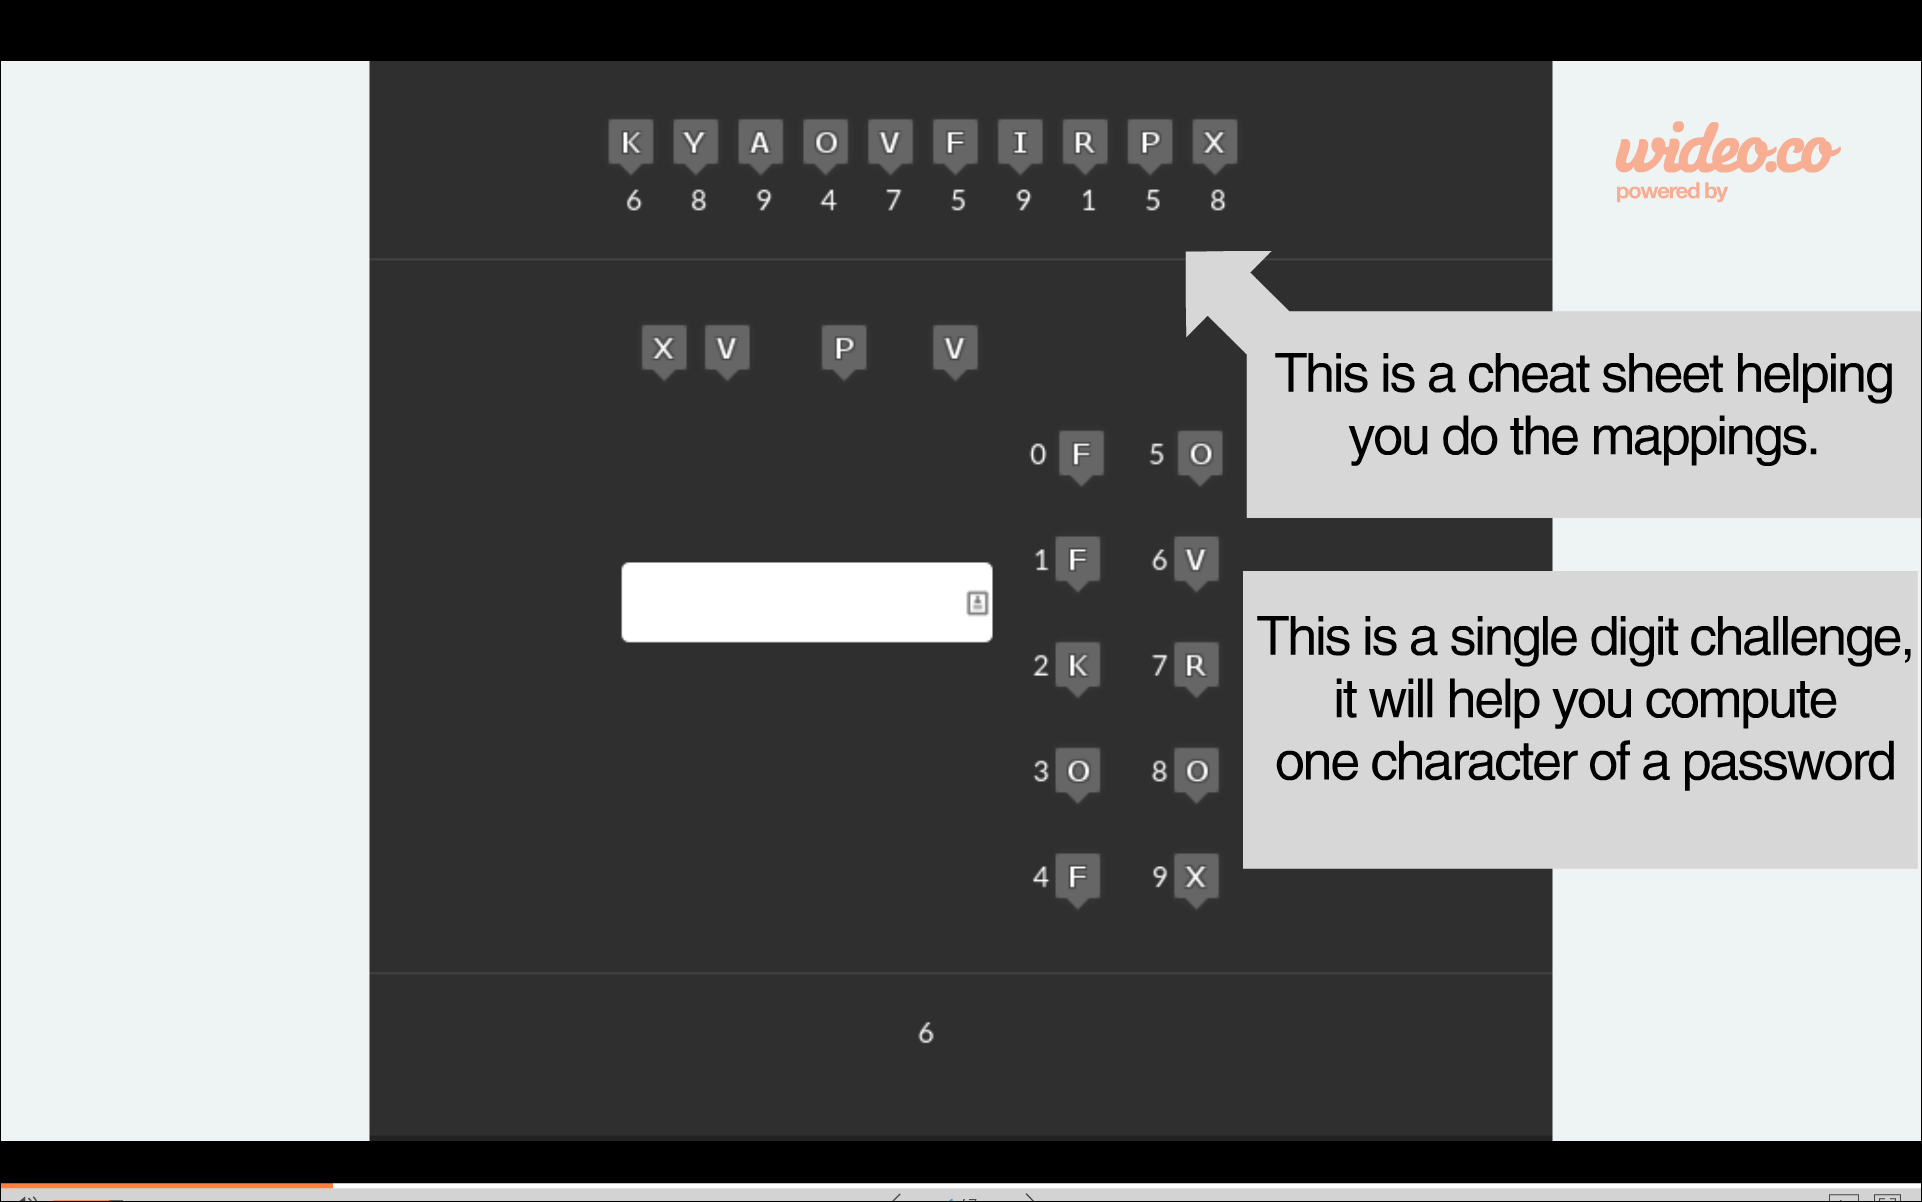
\includegraphics[width=\textwidth]{slides/slide1}
    \caption{Demo slide 1.}
    \label{slide1}
\end{figure}


\begin{figure}
    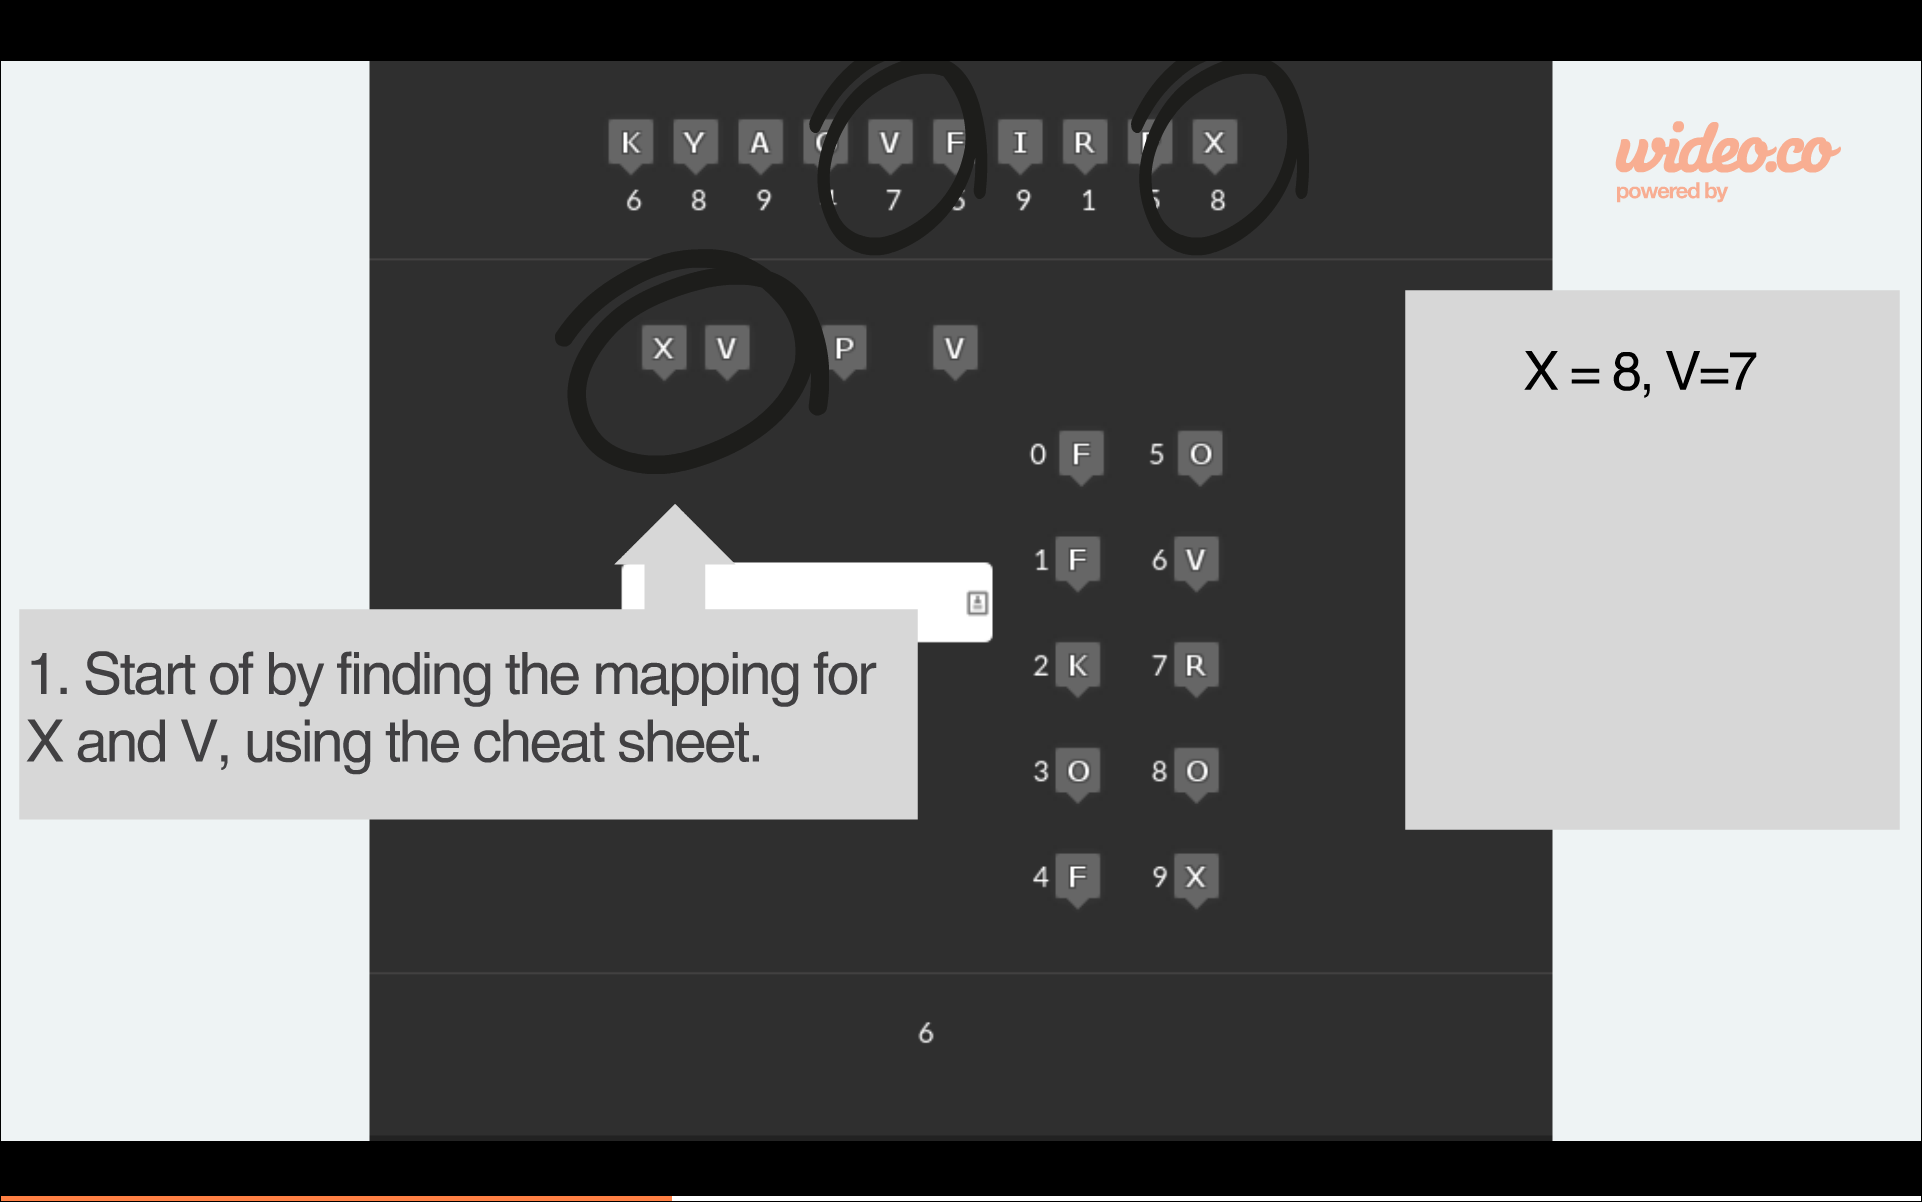
\includegraphics[width=\textwidth]{slides/slide2}
    \caption{Demo slide 2.}
    \label{slide2}
\end{figure}


\begin{figure}
    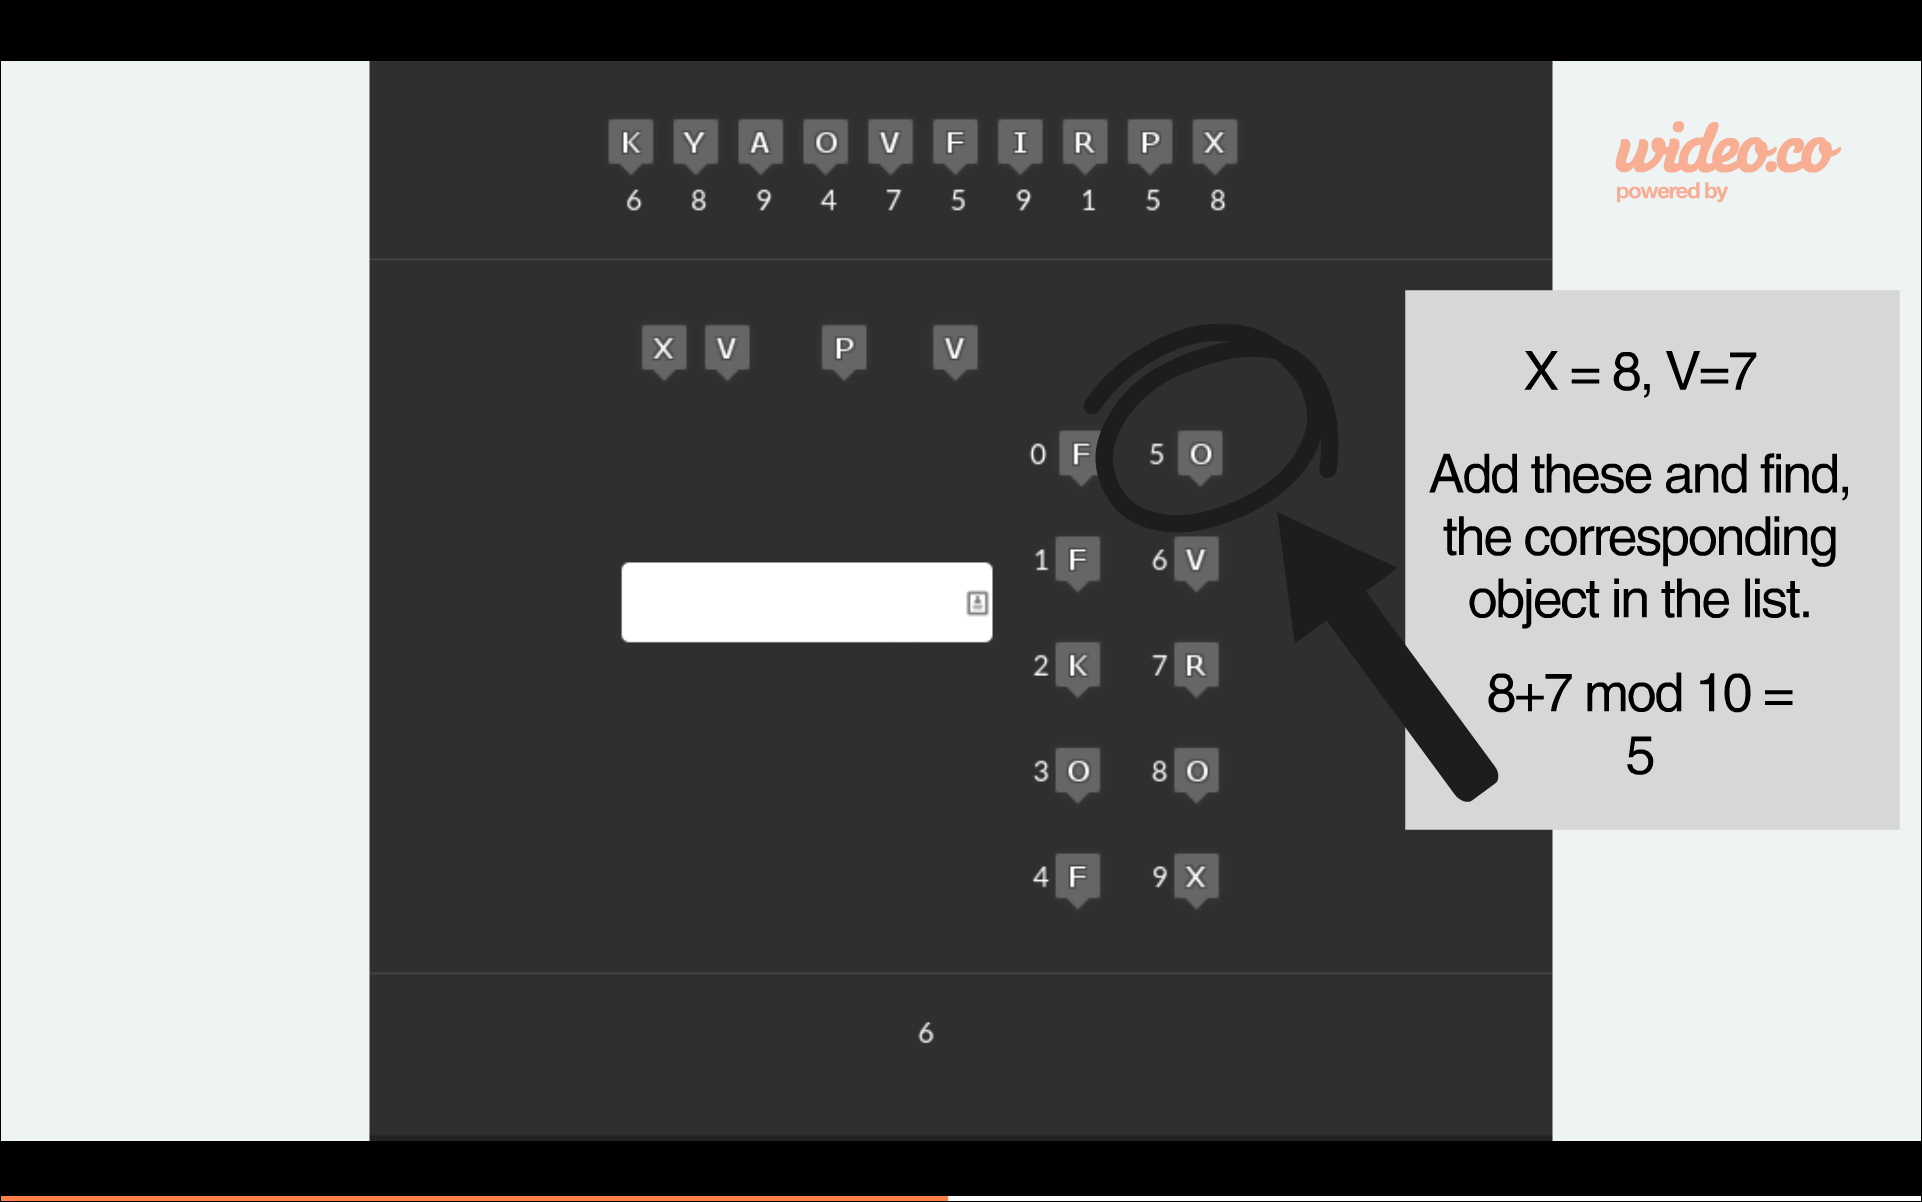
\includegraphics[width=\textwidth]{slides/slide3}
    \caption{Demo slide 3.}
    \label{slide3}
\end{figure}


\begin{figure}
    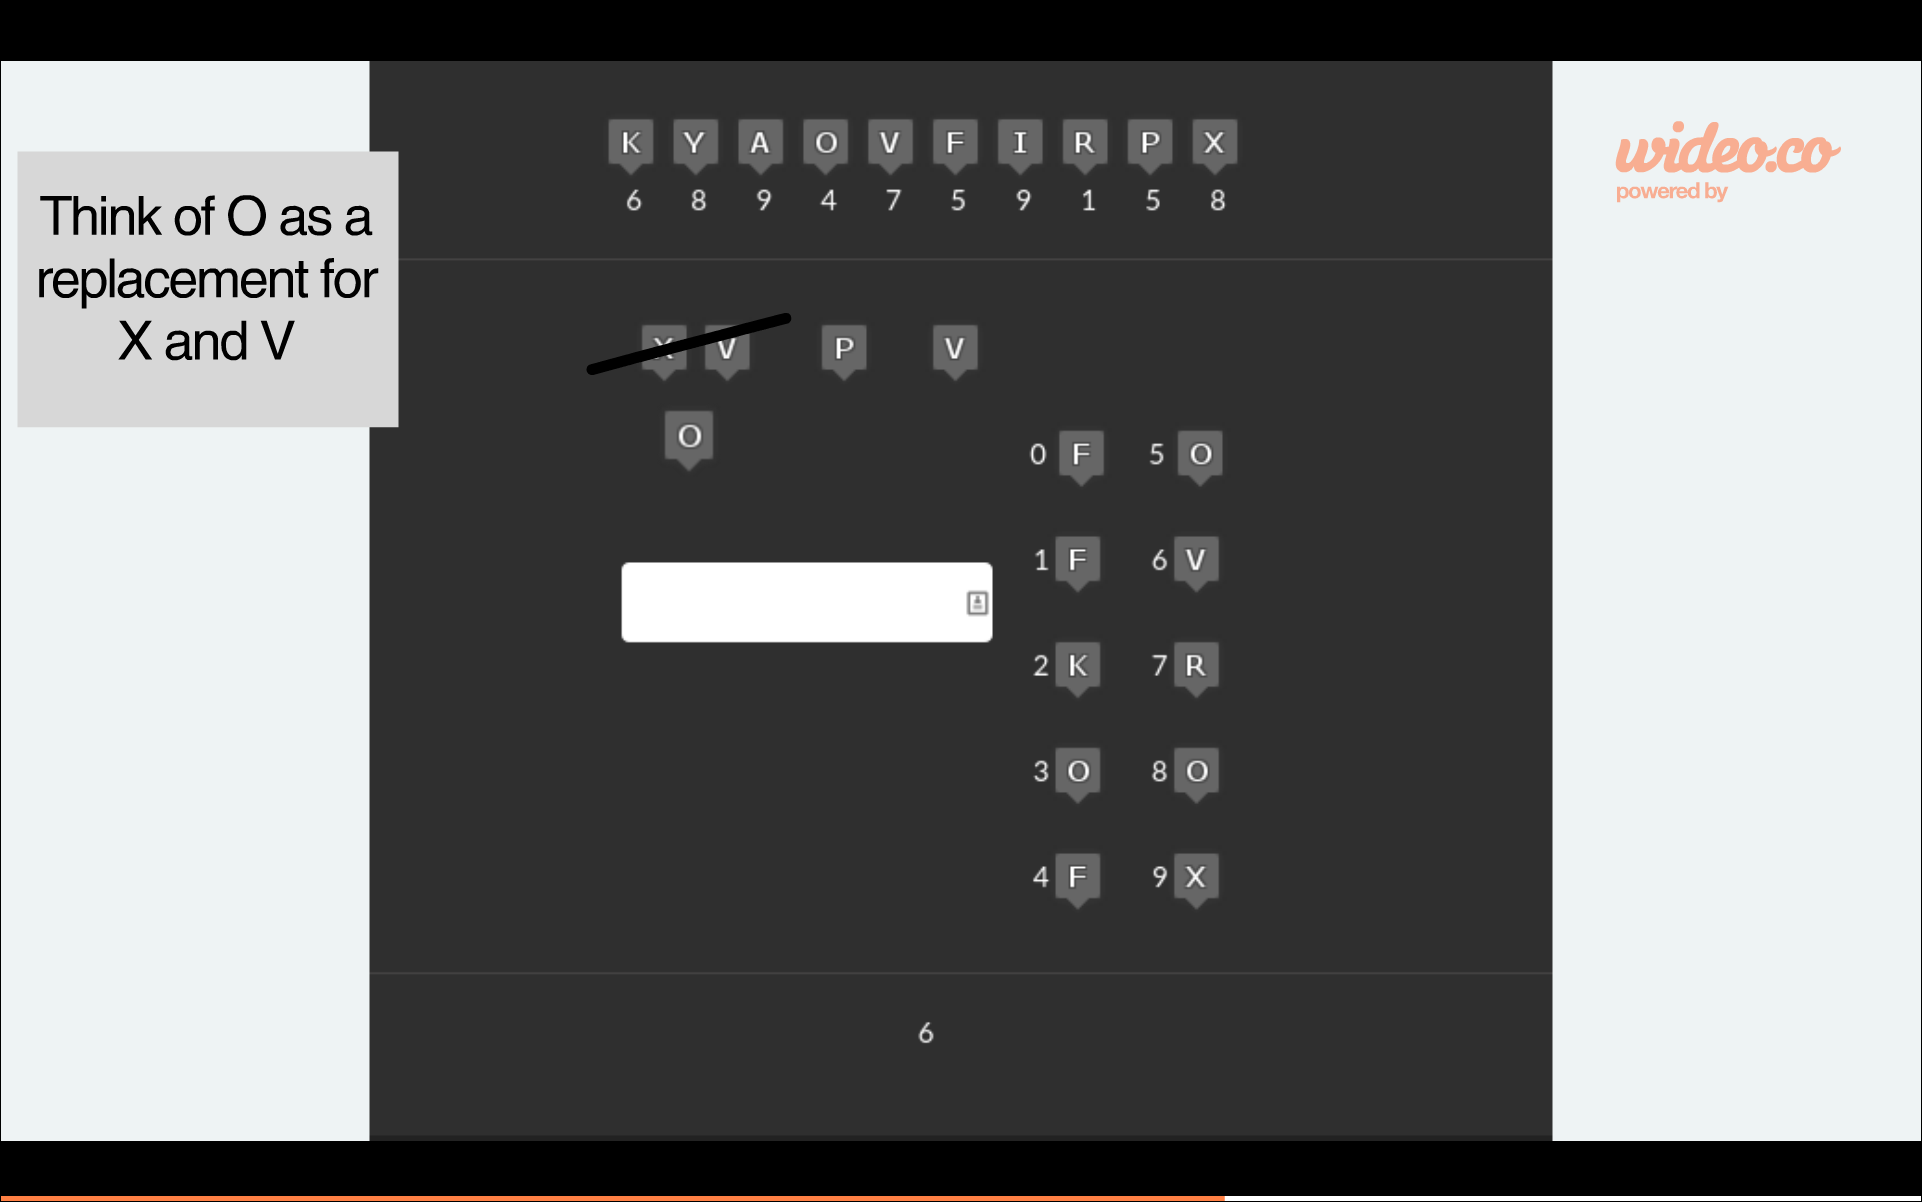
\includegraphics[width=\textwidth]{slides/slide4}
    \caption{Demo slide 4.}
    \label{slide4}
\end{figure}

\begin{figure}
    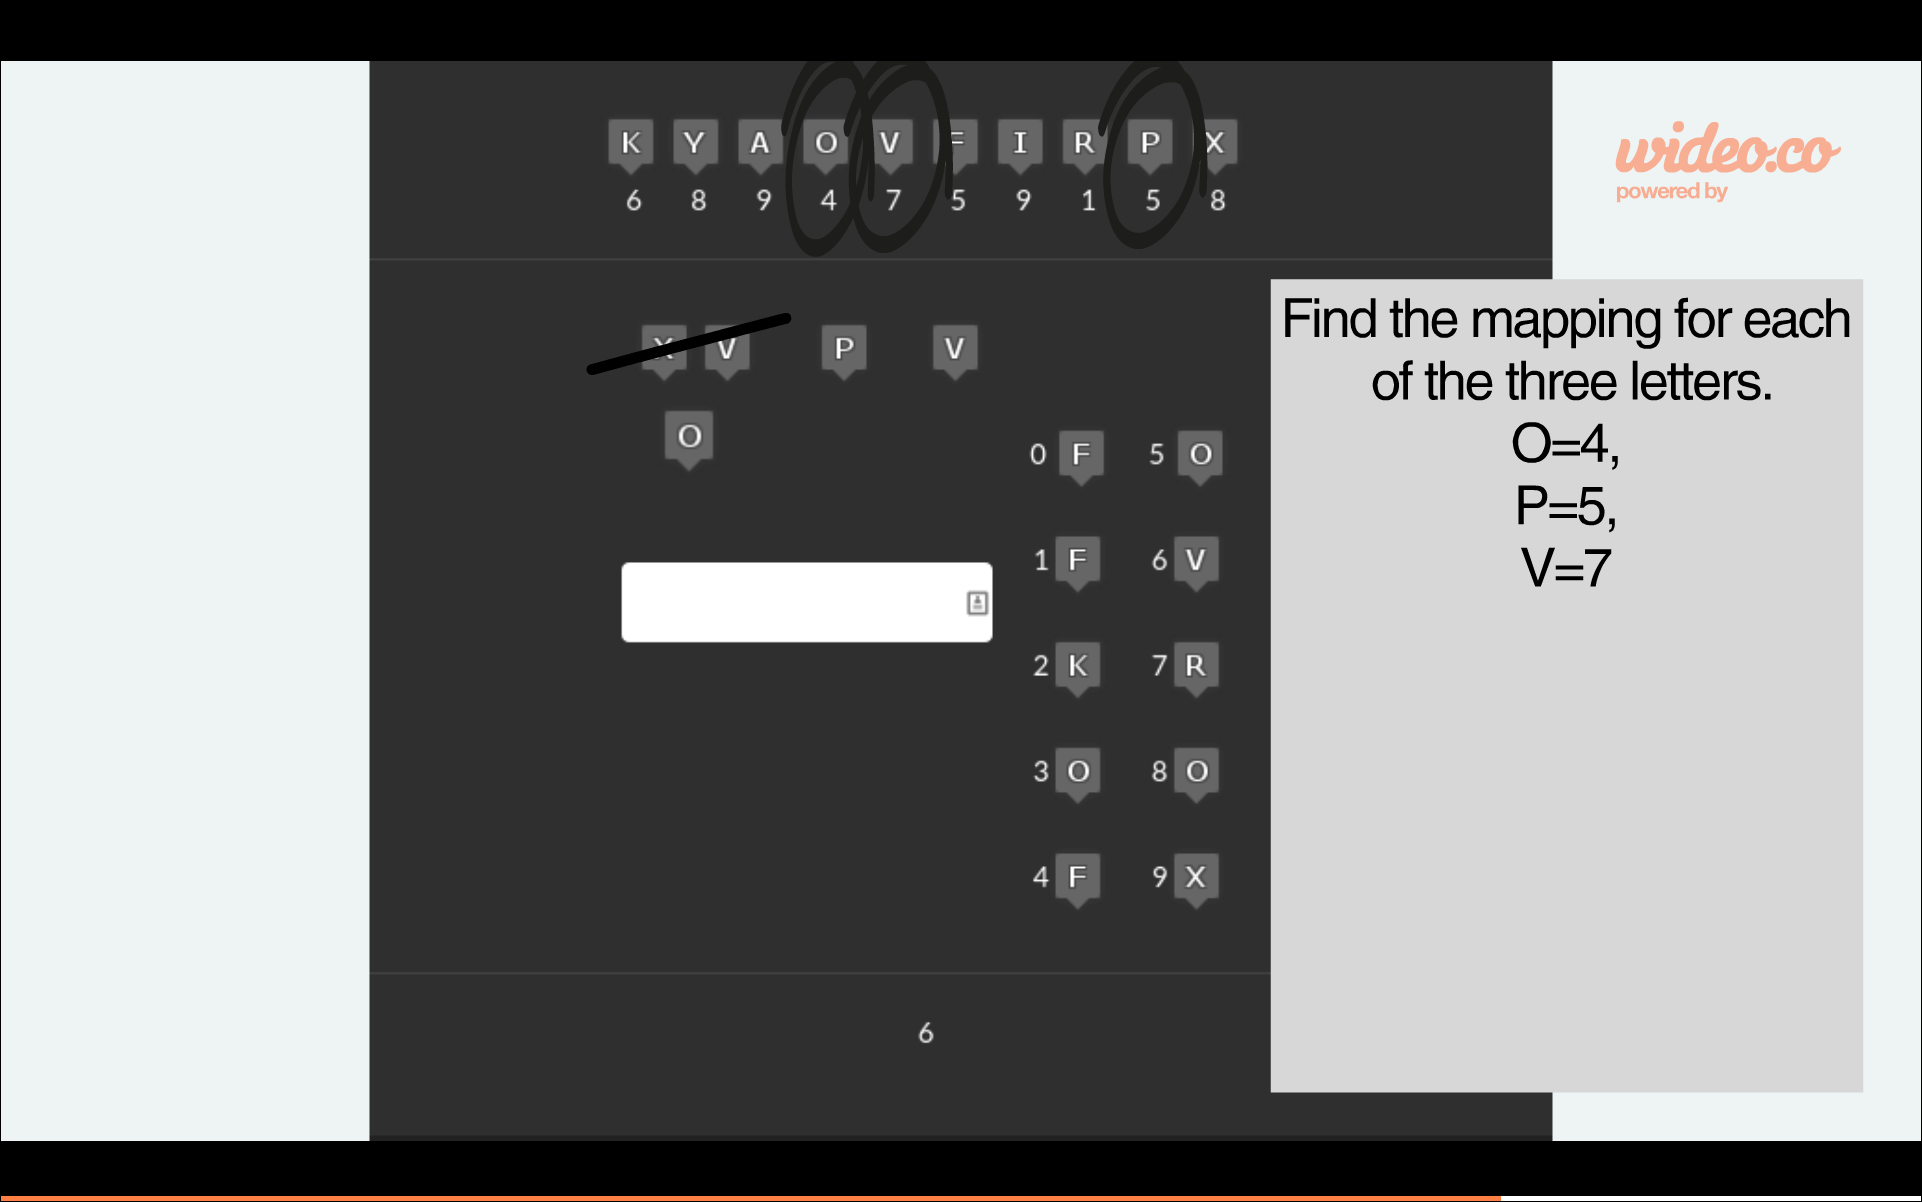
\includegraphics[width=\textwidth]{slides/slide5}
    \caption{Demo slide 5.}
    \label{slide5}
\end{figure}


\begin{figure}
    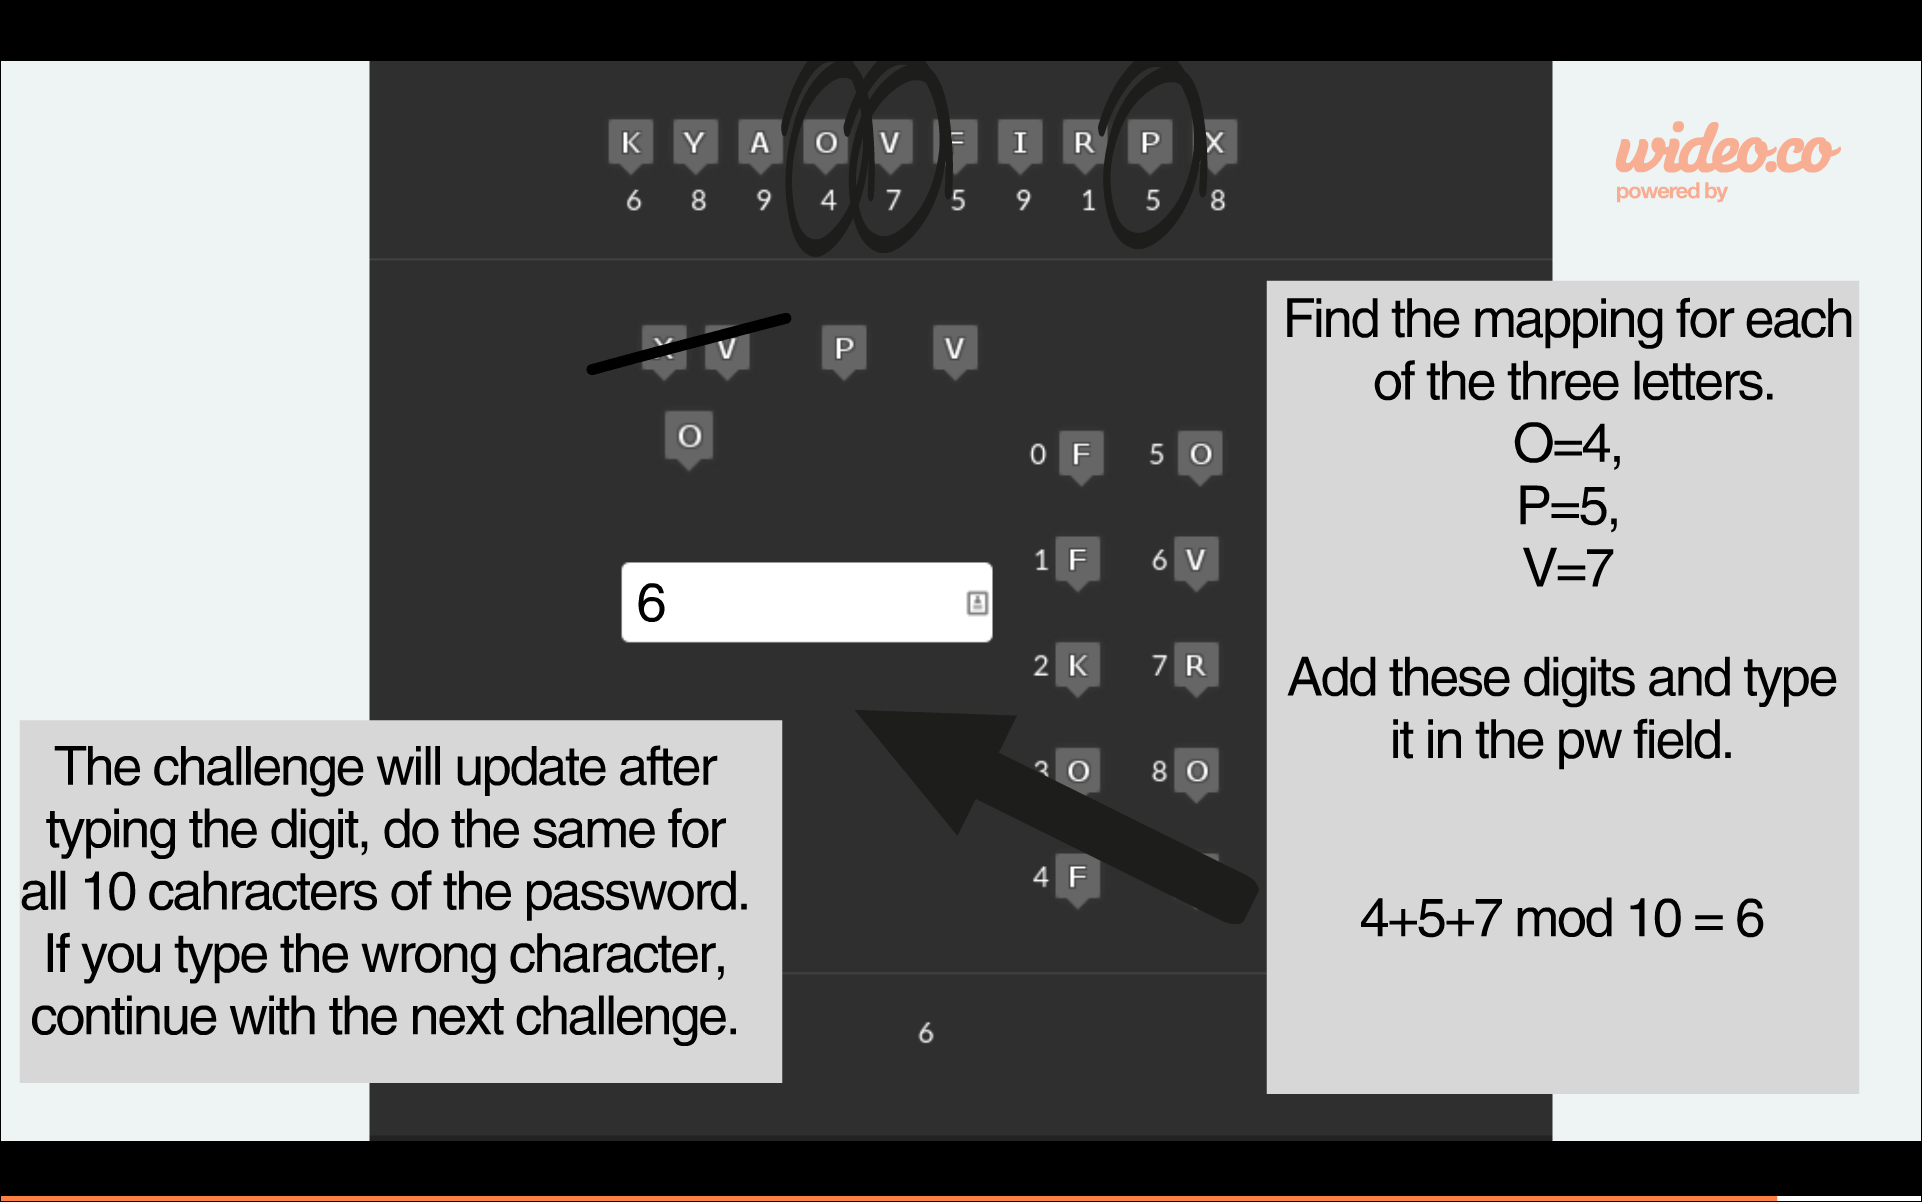
\includegraphics[width=\textwidth]{slides/slide6}
    \caption{Demo slide 6.}
    \label{slide6}
\end{figure}


\chapter{Content Script}\label{app:content-script}

\lstdefinelanguage{JavaScript}{
    keywords={break, case, catch, continue, debugger, default, delete, do, else, finally, for, function, if, in, instanceof, new, return, switch, this, throw, try, typeof, var, void, while, with},
    morecomment=[l]{//},
    morecomment=[s]{/*}{*/},
    morestring=[b]',
    morestring=[b]",
    sensitive=true
}
\lstdefinestyle{jsStyle}{
    language=JavaScript,
    numbers=left,
    stepnumber=1,
    numbersep=10pt,
    tabsize=4,
    showspaces=false,
    showstringspaces=false,
    captionpos=b
}
\lstinputlisting[caption=Content script file., style=jsStyle, basicstyle=\scriptsize]{code/content_script.js}

The content script listines for the onload event triggered by the windows object when a new page is loaded. When receiving this event the updateUrl function(line 27) is called, which sends an update containing the \emph{window.location.hostname} which essentially is the hostname of the current page. Hostname is used since login forms may be located at different locations at different domains.
\par Next the script search the DOM for input fields of type "password" using the \emph{getPwdInputs} function(line 16). This function iterates through all the input fields looking for password fields. If a password field is found, an event listener is attached to the field, listening for events of type "input" which are sent when the field changes\footnote{https://developer.mozilla.org/en-US/docs/Web/API/EventTarget/addEventListener}. When the password field changes a message containing the new length of the password is sent to the controller. 



\end{document} 
